% Anonymous manuscript for double-anonymized review at
% Engineering Applications of Artificial Intelligence.
\documentclass[preprint,12pt,authoryear]{elsarticle}

% Shared packages and layout for the anonymous manuscript and author version.
% The `preprint` elsarticle option is single-column, as required by EAAI.

\usepackage{amsmath}
\usepackage{amssymb}
\usepackage[ruled,vlined]{algorithm2e}

\newlength{\algoblockwidth}
\setlength{\algoblockwidth}{0.82\textwidth}

\usepackage{graphicx}
\graphicspath{{figures/}}
\usepackage{subcaption}
\usepackage{float}
\usepackage{tikz}
\usetikzlibrary{calc,arrows.meta,positioning}

\usepackage{booktabs}
\usepackage{multirow}
\usepackage{array}
\usepackage{tabularx}
\usepackage{longtable}

\usepackage{url}
\usepackage{enumitem}
\usepackage{microtype}
\usepackage{seqsplit}

\biboptions{round,authoryear}

\renewcommand{\topfraction}{0.9}
\renewcommand{\bottomfraction}{0.8}
\renewcommand{\textfraction}{0.07}
\renewcommand{\floatpagefraction}{0.75}

\widowpenalty=10000
\clubpenalty=10000
\displaywidowpenalty=10000



\begin{document}

\begin{frontmatter}

\title{Layout-Preserving Multilingual Translation of Documents in Portable
Document Format with Large Language Models}

% Engineering Applications of Artificial Intelligence uses double-anonymized
% review. Author names, affiliations, acknowledgements and contribution roles
% are therefore supplied only in title_page.tex.

\begin{abstract}
  % Equal-contribution note. The title block is set in a box (see main.tex) and
  % footnotes cannot escape from a box, so the marker is written by hand there
  % and the note itself is emitted here, from ordinary page body.
  \blfootnote{$^{*}$These authors contributed equally to this work.}%
  PDF translation is a joint machine-translation and reconstruction problem:
  pages store positioned glyphs rather than semantic paragraphs, and translated
  text rarely occupies the same visual space as the source. This paper studies
  where errors arise in a layout-preserving PDF translation pipeline and which of
  them its design can control. We hypothesise that document structure analysis is
  a binding stage because its errors are unrecoverable downstream, and that
  layout fidelity is better computed during reconstruction than requested from a
  language model as a length constraint. Our three-stage system parses every page
  visually with layout detection, OCR and table-cell detection, translates
  addressable elements with an identifier-preserving LLM contract, and
  reconstructs the page by estimating font size and appearance from the source
  geometry and pixels. Stage-level evaluation supports this design. On 1{,}651
  OmniDocBench pages, the parser reaches $F_1@.5 = 0.940$ under a
  granularity-invariant matcher and $0.889$ label accuracy; symbol recognition is
  strong (formula CDM $F_1 = 0.863$), so the remaining loss is one of
  \emph{detection}---formulas on three-column pages and roughly a fifth of
  tables---rather than reading. The same shape appears at cell level on
  PubTables-1M, used because OmniDocBench has no per-cell boxes: $F_1 = 0.902$
  overall, but recall of $0.504$ on cells spanning several rows or columns.
  On all 55 \texttt{en}$\rightarrow$\texttt{xx}
  WMT24++ pairs, five LLMs span $0.788$--$0.841$ COMET-DA, with smaller
  between-model than between-language variation. Finally, a $\pm15\%$
  character-length constraint is honoured only 69--73\% of the time and is
  uncorrelated with adequacy ($r = 0.066$). These results are not a substitute
  for an end-to-end PDF benchmark, but they identify the stages and document
  types where such a benchmark should focus.
\end{abstract}


\begin{keyword}
document translation \sep document analysis \sep machine translation \sep
layout reconstruction \sep multilingual documents \sep optical character recognition
\end{keyword}

\end{frontmatter}

\section{INTRODUCTION}
\label{sec:introduction}

\subsection{Background}

The Portable Document Format is the dominant container for
presentation-critical text---textbooks, scientific articles, contracts and
technical reports---precisely because it fixes the visual result: glyph
positions, fonts, tables, mathematical expressions and figures are pinned to a
coordinate system that renders identically on every device~\citep{pdf-spec}.
Over the past decade, considerable research effort has been directed at the two
capabilities that a document translation system must combine. On the one hand,
document layout analysis has matured from heuristic segmentation into a
learned detection problem, supported by large human-annotated corpora such as
DocLayNet~\citep{doclaynet} and by detectors designed for the extreme scale
variation of document pages~\citep{doclayout-yolo}; surveys of the field
consistently report that the quality of this stage propagates directly into
every downstream task~\citep{doclayout-survey}. On the other hand, large
language models (LLMs) have substantially changed machine translation,
particularly for lower-resource pairs and for text that needs domain context.
Unlike neural machine translation systems trained for a fixed set of language
pairs~\citep{nmt-survey}, an LLM is multilingual by construction, can exploit a
wide context window, follows instructions, and can be steered towards
consistent terminology through the prompt~\citep{gpt-mt,llm-multilingual-mt}.
Because most LLMs are consumed through hosted APIs, a document translation
system can now be assembled without training any model of its own.

\subsection{Problem Statement}

The very property that makes PDF attractive makes it hostile to translation. A
PDF page is a stream of drawing operators, not a sequence of paragraphs, so
translating one is simultaneously a machine-translation problem and a
\emph{layout reconstruction} problem. Target text almost never has the length
of the source---Vietnamese and German typically expand relative to English,
while Chinese, Japanese and Korean contract---so writing the translation back
into the original boxes produces overflow, collisions with neighbouring
elements, or font shrinkage severe enough to harm readability. Nor is geometry
the only property that must survive: a translated block inherits the visual
role of the block it replaces, so its typeface, size and \emph{colour}---on
whatever background the source page happens to use---are part of the
reconstruction problem rather than cosmetic detail.

It is tempting to treat the input side as solved. Libraries such as PyMuPDF,
\texttt{pdfminer.six} and \texttt{pdfplumber} read a PDF content stream and
return text almost instantly. In practice they only expose the \emph{text
layer} that happens to be stored in the file, rather than analysing what the
page actually displays, and that layer is unreliable in three recurrent ways.
Scanned PDFs are bitmap images and carry no text layer at all, so optical
character recognition (OCR) is unavoidable. \emph{Searchable} scanned PDFs
carry a hidden OCR layer that may disagree with the visible image, so an
extractor silently returns something other than what the reader sees. And even
in born-digital files, embedded fonts with private encodings, missing
\texttt{ToUnicode} maps, formulas stored as isolated drawing operators and
tables stored as scattered text runs all yield extracted strings that are
corrupted or structurally meaningless.

\subsection{Research Gap}

Which stage of a layout-preserving PDF translation system actually binds its
quality? The question is not rhetorical: its answer decides where design and
research effort belong. Existing systems and document-conversion toolkits have
made substantial progress on different parts of the problem---layout-preserving
overlay for scientific PDFs~\citep{pdf2zh}, document-level segmentation and
terminology~\citep{docutranslate}, OCR-and-rebuild workflows for scanned
input~\citep{retain-pdf}, and PDF-to-structured-output parsers for downstream
LLM use~\citep{docling,marker,mineru,olmocr}. What remains hard to infer from
this literature is not whether these components are useful, but how much each
stage contributes to the failure modes of the final translated document. The
available evidence is difficult to compare directly: some systems export
Markdown or JSON rather than a translated PDF, some prioritise born-digital PDFs
and have limited scanned-document support, and most public evaluations score
either document parsing or plain-text translation rather than the reconstructed
artifact.

Three observations motivate measuring the stages apart. First, \textbf{structure
analysis is lossy in a way translation cannot repair}: a region the parser never
emits is content no downstream model can restore, and a mis-read glyph becomes
the translator's input, so errors here are not additive with translation errors
but place a \emph{ceiling} on the pipeline---yet the stage is almost never scored
against ground truth \emph{as a stage}, because a segmentation error and a
translation error arrive together in the final PDF. Second, \textbf{LLM
translation may be a smaller controllable lever}: a designer chooses
among hosted models but controls neither their training data nor the per-language
resource that dominates their quality, so if competitive models occupy a narrow
band, model selection has little leverage compared with the stages specific to
the document task. Third, \textbf{layout preservation is commonly delegated to
the translator}---instructing the model to keep the target within a length budget
of the source is a widespread device, convenient because it costs nothing at
reconstruction time---yet whether such a budget is honoured, and whether
honouring it relates to quality at all, has not been tested.

\subsection{Hypothesis}
\label{subsec:hypothesis}

This study is organised around a single hypothesis, stated in two parts so that
each part is separately falsifiable.

\paragraph{H1 (the bottleneck).} In layout-preserving PDF translation the
largest controllable headroom may lie in \emph{document structure analysis}
rather than in model choice for translation: the parsing stage can produce
non-recoverable content loss whose incidence is concentrated in identifiable
document slices, whereas competitive LLMs may differ only modestly on the
content that does reach them, and much of the remaining variation may be
explained by the target language rather than by pipeline design.

\paragraph{H2 (where layout must be enforced).} Prompt-level length constraints
are an unreliable proxy for layout fidelity. Even when they influence generation,
they do not tell the system whether rendered text will fit the local geometry of
the page; geometry and appearance must instead be \emph{computed at
reconstruction time from the source page}.

\subsection{The Present Study}

We design and implement a layout-preserving multilingual PDF translation
pipeline whose three stages---document structure analysis, content translation
and document reconstruction---are connected by a single structured intermediate
representation carrying element type, bounding box, page index and reading
order, so that each stage exposes a measurable interface. Two design decisions
follow from the hypothesis. To avoid depending on an embedded text layer that is
absent or unreliable for scanned and searchable-scanned documents, every page is
rendered and analysed visually; the cost of that uniform choice is evaluated at
the parser stage rather than assumed away. To keep layout control in the stage
that can see the page, reconstruction decides both the \emph{size} and the
\emph{colour} of every translated block from the source page itself, rather than
inheriting them from a global default or delegating them to the translator.

The hypothesis is examined through three independent stage-level measurements,
defined in Section~\ref{subsec:method-eval}. A separate final-artifact comparison
is reported in Section~\ref{subsec:res-compliance}.

\begin{description}[leftmargin=0em,labelsep=0.4em,itemsep=0.15em]
  \item[M1] \emph{How much content the parser loses, and where.} The visual
  parsing stage is scored against annotated ground truth on localisation,
  labels, text and reading order, sliced by language, layout and document
  source, with deviations that are \emph{benign} for translation separated from
  those that lose the translator's input---only the latter bound the pipeline
  (H1).
  \item[M2] \emph{How much translation quality depends on model choice.} Five
  LLMs are compared on \texttt{en}$\rightarrow$\texttt{xx} translation over many
  target languages with the pipeline held fixed, contrasting the spread
  \emph{between systems} with the spread \emph{between languages} (H1).
  \item[M3] \emph{Whether a prompt-level length constraint is a useful proxy for
  layout fidelity.} Per-language compliance with the $\pm15\%$ length constraint is
  measured and related to translation quality, contrasting expanding
  (Vietnamese, German) with contracting (CJK) targets (H2).
\end{description}

\subsection{Contributions}

This paper makes three contributions.

\begin{enumerate}[leftmargin=1.4em]
  \item \textbf{A layout-preserving architecture in which reconstruction owns
  geometry and appearance.} Translated text is re-typeset inside the source
  geometry by two decisions computed from the source page rather than from the
  translation: a \emph{size} decision, which derives a canonical font size per
  group of same-role elements from the source text and reduces an individual
  element only when its overflow would actually collide with a neighbour; and a
  \emph{colour} decision, which estimates each element's background from a ring
  of pixels around it and its text colour from the core glyph pixels most
  distant from that background---so the same overlay mechanism serves scanned
  and born-digital pages, and coloured text on non-white backgrounds survives
  translation. Upstream, structurally distinctive content (tables,
  mathematical formulas) is routed through dedicated multimodal verification
  instead of being translated as undifferentiated text
  (Section~\ref{sec:methodology}).

  \item \textbf{A stage-level evaluation protocol that makes parsing
  measurable.} We score the parsing stage directly on positions, labels, text
  and reading order against OmniDocBench~\citep{omnidocbench} instead of
  collapsing its output to Markdown, which would discard exactly the geometric
  information the task depends on, and we report a strict and a
  granularity-invariant matcher \emph{as a pair} so that a deliberate design
  choice is not misread as a detection defect; cell geometry, which OmniDocBench
  cannot support, is scored on PubTables-1M~\citep{pubtables1m}; translation is
  scored on all 55
  language pairs of WMT24++~\citep{wmt24pp} with five LLMs, keeping the
  document-level translation protocol intact
  (Sections~\ref{sec:methodology} and~\ref{sec:results}).

  \item \textbf{Stage-level evidence for H1 and H2.} We show that the dominant
  parser error is benign over-segmentation rather than missed content, but that
  the residual content loss is concentrated and non-recoverable (over half of
  the formulas on three-column pages, one table in five); that the quality
  spread between five LLMs on a fixed language ($\approx 0.05$ COMET-DA) is
  roughly a third of the spread attributable to per-language resource
  ($\approx 0.18$), which script family alone does not explain; and that a
  character-based length constraint is honoured only 69--73\% of the time and is
  essentially uncorrelated with semantic adequacy ($r = 0.066$), i.e.\ it
  measures script density rather than quality (Sections~\ref{sec:results}
  and~\ref{sec:discussion}).
\end{enumerate}

The remainder of the paper is organised as follows.
Section~\ref{sec:literature} reviews the PDF layout problem, the model
families the pipeline builds on, and related translation and document-conversion
systems.
Section~\ref{sec:methodology} presents the proposed architecture and the
experimental design of both evaluations. Section~\ref{sec:results} reports the
results, Section~\ref{sec:discussion} interprets them against H1 and H2 and
states the limitations, and Section~\ref{sec:conclusion} concludes.

\section{LITERATURE REVIEW}
\label{sec:literature}

This section narrows from the format itself to the systems the proposed pipeline
is positioned against. We first make explicit the mismatch between the
presentational structure of PDF and the semantic structure machine translation
requires (Section~\ref{subsec:lit-pdf}); we then review the model families the
pipeline builds on (Section~\ref{subsec:lit-models}); next we distinguish
document-conversion systems from document-translation systems
(Sections~\ref{subsec:lit-conversion} and~\ref{subsec:lit-systems}); and finally
we state the gap that motivates the hypothesis of Section~\ref{subsec:hypothesis}
and the design decisions of Section~\ref{sec:methodology}
(Section~\ref{subsec:lit-gap}).

\subsection{PDF Structure and Layout Preservation}
\label{subsec:lit-pdf}

\paragraph{Format characteristics.} Under ISO~32000-2, page content is a stream
of graphics operators that place glyphs, strokes and images into a fixed
coordinate system~\citep{pdf-spec}. This is appropriate for display and print,
but it does not guarantee that semantic units---headings, paragraphs, table
cells, reading order---can be recovered directly. With respect to content
accessibility, PDF documents fall into three groups. \emph{Born-digital} files
contain text objects with font and position information, and can be extracted
directly, although the order in which objects appear in the content stream need
not be the reading order. \emph{Scanned} files contain page bitmaps and no
trustworthy text layer, and therefore require OCR. \emph{Mixed} documents
contain born-digital text, scanned pages and text-bearing images at the same
time, so the extraction strategy must be decided per page rather than per
document.

Consequently, raw extraction is not sufficient input for machine translation.
An intermediate representation must record content, element type, bounding box,
page number and reading-order relations simultaneously; it is the bridge
between the semantic domain of translation and the geometric domain of
typesetting.

\paragraph{Element types and per-type policy.} Document layout analysis (DLA)
assigns positions and semantic labels to page regions. Datasets such as
DocLayNet provide bounding-box labels for many element types across diverse
document domains and thus support both training and
evaluation~\citep{doclaynet}, and surveys report that DLA quality directly
determines downstream information extraction, reading-order recovery and format
conversion~\citep{doclayout-survey}. For translation, each element group
requires a distinct policy: flowing text must be grouped into units with enough
context; formulas must preserve their symbols, with only the accompanying prose
translated; figures are copied unchanged while their captions are translated;
and table content must remain bound to the correct row and column, since
translating the flattened string of a table destroys inter-cell relations.

\paragraph{Text overflow.} The length and typesetting behaviour of a
translation differ from those of the source by an amount that depends on the
language pair, the content, the terminology, the font and the line-breaking
rules; a character count alone therefore does not predict the display space
required. When target text is placed into the original box, three failures
appear: content spills outside the box, it overlaps a neighbouring element, or
the font is reduced until legibility suffers. This creates a trade-off between
geometric fidelity and readability. Preserving coordinates and box sizes
exactly keeps the target page close to the source but maximises overflow risk;
re-flowing the page lets text adapt but moves figures, tables and page breaks.
A layout-preserving system must therefore combine several signals---box size,
source typography, surrounding free space, and the possibility of collision
with other elements---and its evaluation must consider layout similarity,
overlap count and readability rather than merely whether an output file was
produced.

\paragraph{Appearance beyond geometry.} Placing target text at the right
coordinates is necessary but not sufficient, because the replaced text also
carried a visual identity. Two properties are routinely lost. First, the
\emph{background}: writing a translation over a source page requires masking
what was there, and masking with a global white rectangle is correct only for
white pages---on coloured slides, textbook sidebars, shaded table rows or
scanned paper the mask is itself a visible defect. Second, the \emph{text
colour}: headings, hyperlinks, emphasised terms and slide text are frequently
non-black, and a reconstruction that repaints everything in black silently
discards a layer of document semantics. Neither property can be read reliably
from the content stream in the general case---scanned pages have no text objects
at all, and born-digital pages express colour through nested graphics
states~\citep{pdf-spec}---so a pipeline that already rasterises every page has
the option, largely unexploited in existing systems, of \emph{estimating}
appearance from the rendered pixels.

\subsection{Foundation Models for Document Analysis}
\label{subsec:lit-models}

A layout-preserving translation pipeline must coordinate a document vision
model, an OCR model, a translation model and a service-orchestration layer.
These components do not operate independently: a recognition error at the front
of the pipeline propagates into the translation and finally manifests as a
typesetting defect. Model selection must therefore weigh accuracy, language
coverage, inference cost, and---critically---whether the output format is usable
by the following stage.

\paragraph{Layout detection.} A layout detector consumes a page image and
returns regions with semantic labels and confidences. DocLayout-YOLO balances
accuracy against speed using diverse synthetic pre-training data and a
global-to-local perception mechanism, which suits document pages where a
one-line heading and a near-full-page table can co-occur~\citep{doclayout-yolo}.
Surya provides layout detection, reading-order estimation and table recognition
inside a single toolkit~\citep{surya}. For our pipeline the important output is
not only the class label but a stable bounding box and a reading order that can
be joined reliably with OCR results.

\paragraph{OCR for scanned PDFs.} A document OCR workflow typically detects
text lines or regions, recognises character sequences, and maps the result back
into page coordinates. Unlike OCR intended only for search, reconstructing a
PDF additionally requires line- or word-level boxes, recognition confidences
and the relation between text and layout regions. Surya supports multilingual
recognition, line detection, reading order, layout, tables and formulas in one
toolkit~\citep{surya}; PaddleOCR contributes multilingual recognition models and
structured document components, which are convenient for table-cell
information~\citep{paddleocr}. No single model is accurate on every document
type: resolution, skew, background noise, typeface and inline formulas all
degrade results. A pipeline must therefore normalise coordinate systems, retain
confidences and keep stable identifiers per element so that errors remain
diagnosable across stages.

\paragraph{Evaluation metrics.} For translation, lexical metrics such as
BLEU~\citep{bleu} and chrF~\citep{chrf} measure surface overlap, whereas neural
metrics such as COMET~\citep{comet} encode source, hypothesis and reference with
a multilingual encoder and regress a continuous adequacy score. The WMT metrics
shared task reports that neural metrics correlate better with human judgement
and are more robust than lexical ones~\citep{wmt-metrics-shared-task}, which is
why we treat COMET as primary and chrF++ as a diagnostic baseline. For document
parsing, OmniDocBench provides 1{,}651 richly annotated pages together with a
composite score built from text edit distance, table TEDS and formula
CDM~\citep{omnidocbench}; CDM itself scores a formula by rendering it and
matching detected symbols, which makes it invariant to notation differences
that penalise string-based metrics unfairly~\citep{cdm}. Most of the string
metrics used below reduce to the Levenshtein edit
distance~\citep{levenshtein}.

\subsection{Document Parsing and Conversion Systems}
\label{subsec:lit-conversion}

Several recent systems address the front half of the problem: turning PDFs into
machine-readable structured representations. Docling converts PDFs into a
document model that can be exported to Markdown or JSON, combining layout
analysis and table-structure recognition in a resource-conscious
package~\citep{docling}. Marker similarly targets Markdown, JSON, HTML and chunk
outputs, using Surya-based OCR and layout models with optional LLM correction for
tables, inline mathematics and block-level repair~\citep{marker}. MinerU focuses
on high-precision document content extraction across diverse layouts, including
tables, formulas and scanned or garbled PDFs~\citep{mineru}. olmOCR takes a
large-scale VLM route, linearising PDFs into clean text while preserving reading
order and structured content for language-model data pipelines~\citep{olmocr}.

These systems are important comparators for the \emph{parsing} side of this
work, and they motivate treating structure analysis as a first-class component
rather than a utility function. They are not, however, direct baselines for the
complete task studied here. Their primary outputs are structured text
representations, not translated PDFs composited back onto the source page; they
optimise readability, retrieval or data preparation rather than preservation of
the original page geometry after translation. A fair end-to-end comparison would
therefore require an additional reconstruction layer on top of each converter,
plus an annotated PDF benchmark that scores both translation adequacy and final
visual fidelity. In the absence of such a benchmark, the present paper compares
the parsing stage to public ground truth and treats direct system-level
comparison as future work rather than evidence of superiority.

\subsection{Related Document Translation Systems}
\label{subsec:lit-systems}

Document translation systems can be distinguished by the intermediate
representation they adopt: coordinate-based representations favour geometric
fidelity, structured-text representations favour context and editability, and
re-typesetting representations rebuild the document from recognised components.
The comparison below concerns published architecture and scope, and does not
treat feature count as evidence of output quality. The systems are discussed
qualitatively because their public implementations do not expose the same input
scope and output contract on scanned, mixed and born-digital PDFs.

\paragraph{Layout preservation by text overlay.} PDFMathTranslate~\citep{pdf2zh}
implements layout detection, content extraction, translation and document
reconstruction. A layout model separates text from regions that must be
preserved, and the text is passed to an intermediate layer supporting several
translation services; target content is written back using the geometry of the
source, so figures, formulas and page structure are disturbed far less than in
a plain-text conversion. The important contribution is the separation of the
layout pipeline from the translation service, which allows the language model to
be replaced without redesigning the PDF parser. Output quality nevertheless
remains bounded by layout-detection accuracy and by the ability to fit
new-length text into old regions, and the published version identifies
suboptimal OCR support as a limitation, which restricts applicability to
scanned PDFs~\citep{pdf2zh}.

\paragraph{Segmentation and terminology consistency.}
docutranslate~\citep{docutranslate} approaches the task from the content side:
it supports many formats, splits content into segments compatible with model
input limits, executes translation asynchronously and supplies a glossary.
Terminology constraints matter particularly for long documents, where the same
concept must be rendered consistently across segments that are never processed
in the same call; their effect has been studied in machine
translation~\citep{terminology-mt}, and recent work on document-level
translation reports that fusing several knowledge sources improves contextual
consistency~\citep{doc-mt-multi-knowledge}. For PDF input, docutranslate uses a
document parser to recognise tables, formulas and code, then converts content to
Markdown before translation. This normalisation is convenient for semantic
processing and multi-format export, but the project documentation states that
the original PDF layout is lost in the conversion~\citep{docutranslate}.

\paragraph{Re-typesetting from OCR.} RetainPDF~\citep{retain-pdf} represents the
OCR-and-rebuild direction, covering content recognition, translation, diagnosis
and PDF export, with an input scope that includes image-only and scanned
documents. Compared with exploiting the existing text layer, this yields a more
uniform representation of born-digital and scanned PDFs and allows control over
fonts, tables and formulas during typesetting. In exchange, rebuilding from OCR
introduces a chain of accumulated error: mis-detected regions produce wrong
reading order, mis-recognised characters change the translation input, and
geometric drift affects placement at export time. As the system is described
mainly through its source repository rather than a peer-reviewed empirical
study, its quality claims require verification on a common dataset and a common
metric set before direct comparison.


\begin{table}[H]
    \centering
    \caption{Qualitative comparison of related document translation approaches.}
    \label{tab:related-work-comparison}
    \footnotesize
    % Fixed 2.6cm + 3x4.0cm columns were set for the 6.75in two-column measure
    % and now overrun the text block; X columns divide whatever measure is in
    % force, so the table fits by construction.
    \begin{tabularx}{\textwidth}{@{}
        >{\raggedright\arraybackslash}p{2.3cm}
        >{\raggedright\arraybackslash}X
        >{\raggedright\arraybackslash}X
        >{\raggedright\arraybackslash}X@{}}
        \toprule
        \textbf{Criterion} & \textbf{PDFMathTranslate} & \textbf{docutranslate} & \textbf{RetainPDF} \\
        \midrule
        Representation
        & Bound to the source PDF
        & Markdown or format-specific structure
        & Re-typeset PDF \\
        Primary objective
        & Preserve formulas and page layout
        & Translation context, terminology, many formats
        & Support image/scanned PDF and re-export \\
        Stated limitation
        & OCR support suboptimal in the published version
        & PDF-to-Markdown conversion loses the original layout
        & Error may accumulate through OCR and rebuilding \\
        Published evidence
        & Peer-reviewed system paper
        & Documentation and source repository
        & Documentation and source repository \\
        \bottomrule
    \end{tabularx}
\end{table}

\subsection{Synthesis and Research Gap}
\label{subsec:lit-gap}

The systems above are not mutually exclusive; they optimise different
objectives. PDFMathTranslate prioritises the geometric layout of born-digital
PDFs, docutranslate prioritises a content representation convenient for
document-level translation, RetainPDF extends coverage to scanned documents
through OCR and reconstruction, and document-conversion systems such as
Docling, Marker, MinerU and olmOCR prioritise high-quality structured extraction
for downstream applications. Table~\ref{tab:related-work-comparison} summarises
the differences drawn from published papers and project documentation.

The gap should therefore not be phrased as a single missing feature---several
tools already support scanned PDFs, structured extraction or layout-aware export
to varying degrees. What is still under-measured is the \emph{joint} problem of
translation, geometry and appearance: the translated content must remain linked
to page coordinates, and the reconstruction stage must be evaluated as part of
the task rather than treated as a cosmetic post-process. Four requirements are
therefore not addressed simultaneously by the surveyed systems:

\begin{itemize}[leftmargin=1.2em]
  \item \textbf{Unified input handling.} Born-digital, scanned and mixed PDFs
  should follow one processing path while the provenance of each extracted
  result remains traceable.
  \item \textbf{Joint semantics and geometry.} Segmentation and glossaries
  improve translation consistency, but the translated content must be mapped
  back onto individual geometric elements rather than existing only as text.
  \item \textbf{Page-aware overflow handling.} Uniform shrinking degrades
  readability, while unconstrained overflow produces overlap. The scaling
  decision must depend on whether a collision with a neighbouring element would
  actually occur---which the translator, having no access to the page, cannot
  determine.
  \item \textbf{Appearance fidelity.} A translated block must inherit the
  background it sits on and the colour it is drawn in. Neither is available from
  the content stream for scanned input, so both have to be estimated from the
  rendered page if the output is to remain faithful on anything other than
  black-on-white documents.
\end{itemize}

Two consequences follow, and they structure the rest of the paper. First, because
the surveyed tools report evidence in different forms, no conclusion about which
stage limits output quality can be drawn from feature descriptions alone. That
question must first be approached by measuring the stages apart, which is the
protocol of Section~\ref{subsec:method-eval} and the substance of hypothesis~H1.
Second, because layout preservation is a property of the page rather than of the
text, the requirements above are discharged at reconstruction time, which is
hypothesis~H2 and the substance of Section~\ref{subsec:method-render}.

\section{METHODOLOGY}
\label{sec:methodology}

We describe the implemented pipeline first
(Sections~\ref{subsec:method-overview}--\ref{subsec:method-render}) and then
the stage-level evaluations used to test the hypotheses
(Section~\ref{subsec:method-eval}).

\subsection{System Overview}
\label{subsec:method-overview}

The system processes each PDF through three stages connected by a single JSON
intermediate representation (Figure~\ref{fig:pipeline-overview}). This separation
is methodological as well as
engineering: H1 asks which stage binds quality, so the parser, translator and
reconstructor must each expose an output that can be inspected and scored.

\begin{figure}[tb]
    \centering
    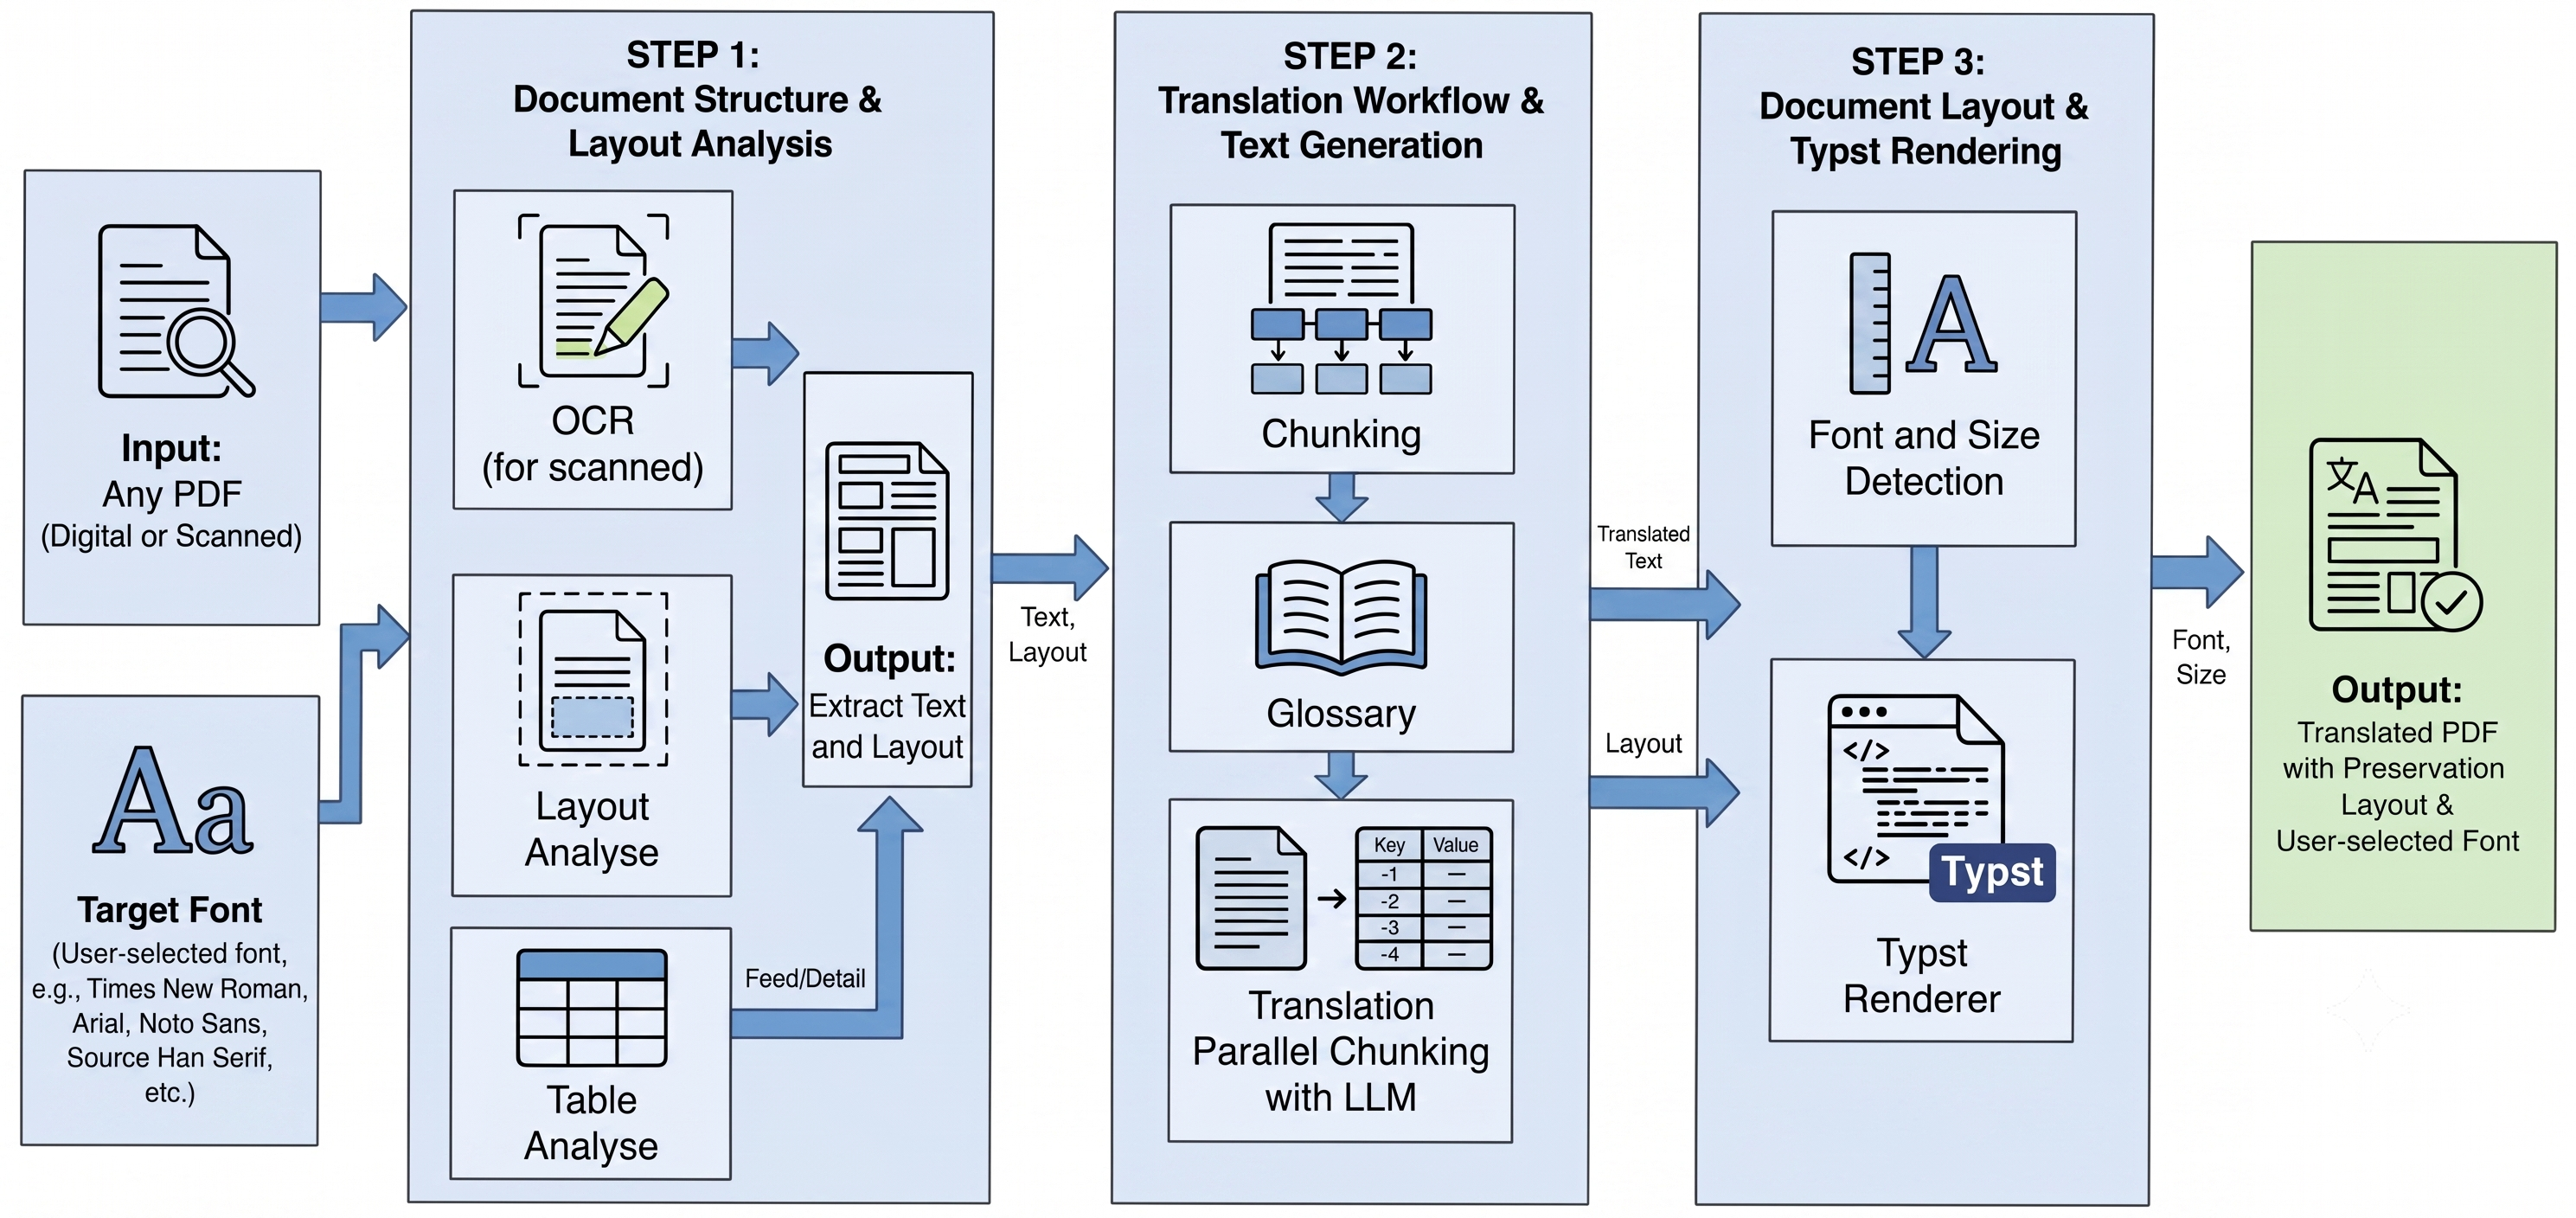
\includegraphics[width=0.9\textwidth]{overview_architect.png}
    \caption{The three-stage pipeline. Each stage consumes the previous
    artifact and writes a new JSON/PDF artifact into a per-session working
    directory, so individual stages can be inspected, corrected or re-run.}
    \label{fig:pipeline-overview}
\end{figure}

\begin{description}[leftmargin=0em,labelsep=0.4em]
  \item[Stage~1 --- Structure analysis.] The source PDF is rendered page by page
  and analysed visually. The output is a \texttt{ParsedDocument} whose elements
  carry page index, bounding box, type label, OCR text, reading order and, for
  tables, cell boxes.
  \item[Stage~2 --- Content translation.] Translatable elements are packed in
  document order and translated by an LLM under an identifier-preserving
  contract, with dedicated handling for tables, formulas and terminology.
  \item[Stage~3 --- Reconstruction.] Translated strings are placed back on the
  source page. Font size is decided from source geometry and local collisions;
  background and text colour are estimated from source pixels before the overlay
  is composited onto the original PDF.
\end{description}

\paragraph{Human-in-the-loop checkpoints.} The prototype exposes two optional
checkpoints: after Stage~1, users can correct labels, OCR text, bypass flags and
table-cell text; after Stage~3, they can edit text on the rendered page. These
checkpoints are not included in the automatic evaluation, but they target the
same unrecoverable errors analysed in Section~\ref{sec:results}.

\subsection{Stage 1: Document Structure Analysis}
\label{subsec:method-parser}

The parser deliberately ignores the embedded text layer and treats every page as
an image. This gives one path for born-digital, scanned and mixed PDFs, avoiding
the common failure in which a hidden OCR layer or broken font encoding differs
from what the reader sees.

\subsubsection{Models and Output Representation}

Four models are used in three modules. Surya Layout predicts page regions and
labels; Surya Text Detection localises text lines; Surya Text Recognition reads
their content; and a PaddleOCR RT-DETR table-cell detector identifies cell boxes
inside table regions~\citep{surya,paddleocr}; detected cell boxes are kept as
geometry for cell-wise translation (Figure~\ref{fig:table-cells}). OCR is run before layout
post-processing so its line boxes can tighten regions, split sparse blocks and
recover missed text (Figure~\ref{fig:parser-stages}).

\begin{figure}[H]
  \centering
  \begin{subfigure}[t]{0.25\textwidth}
    \centering
    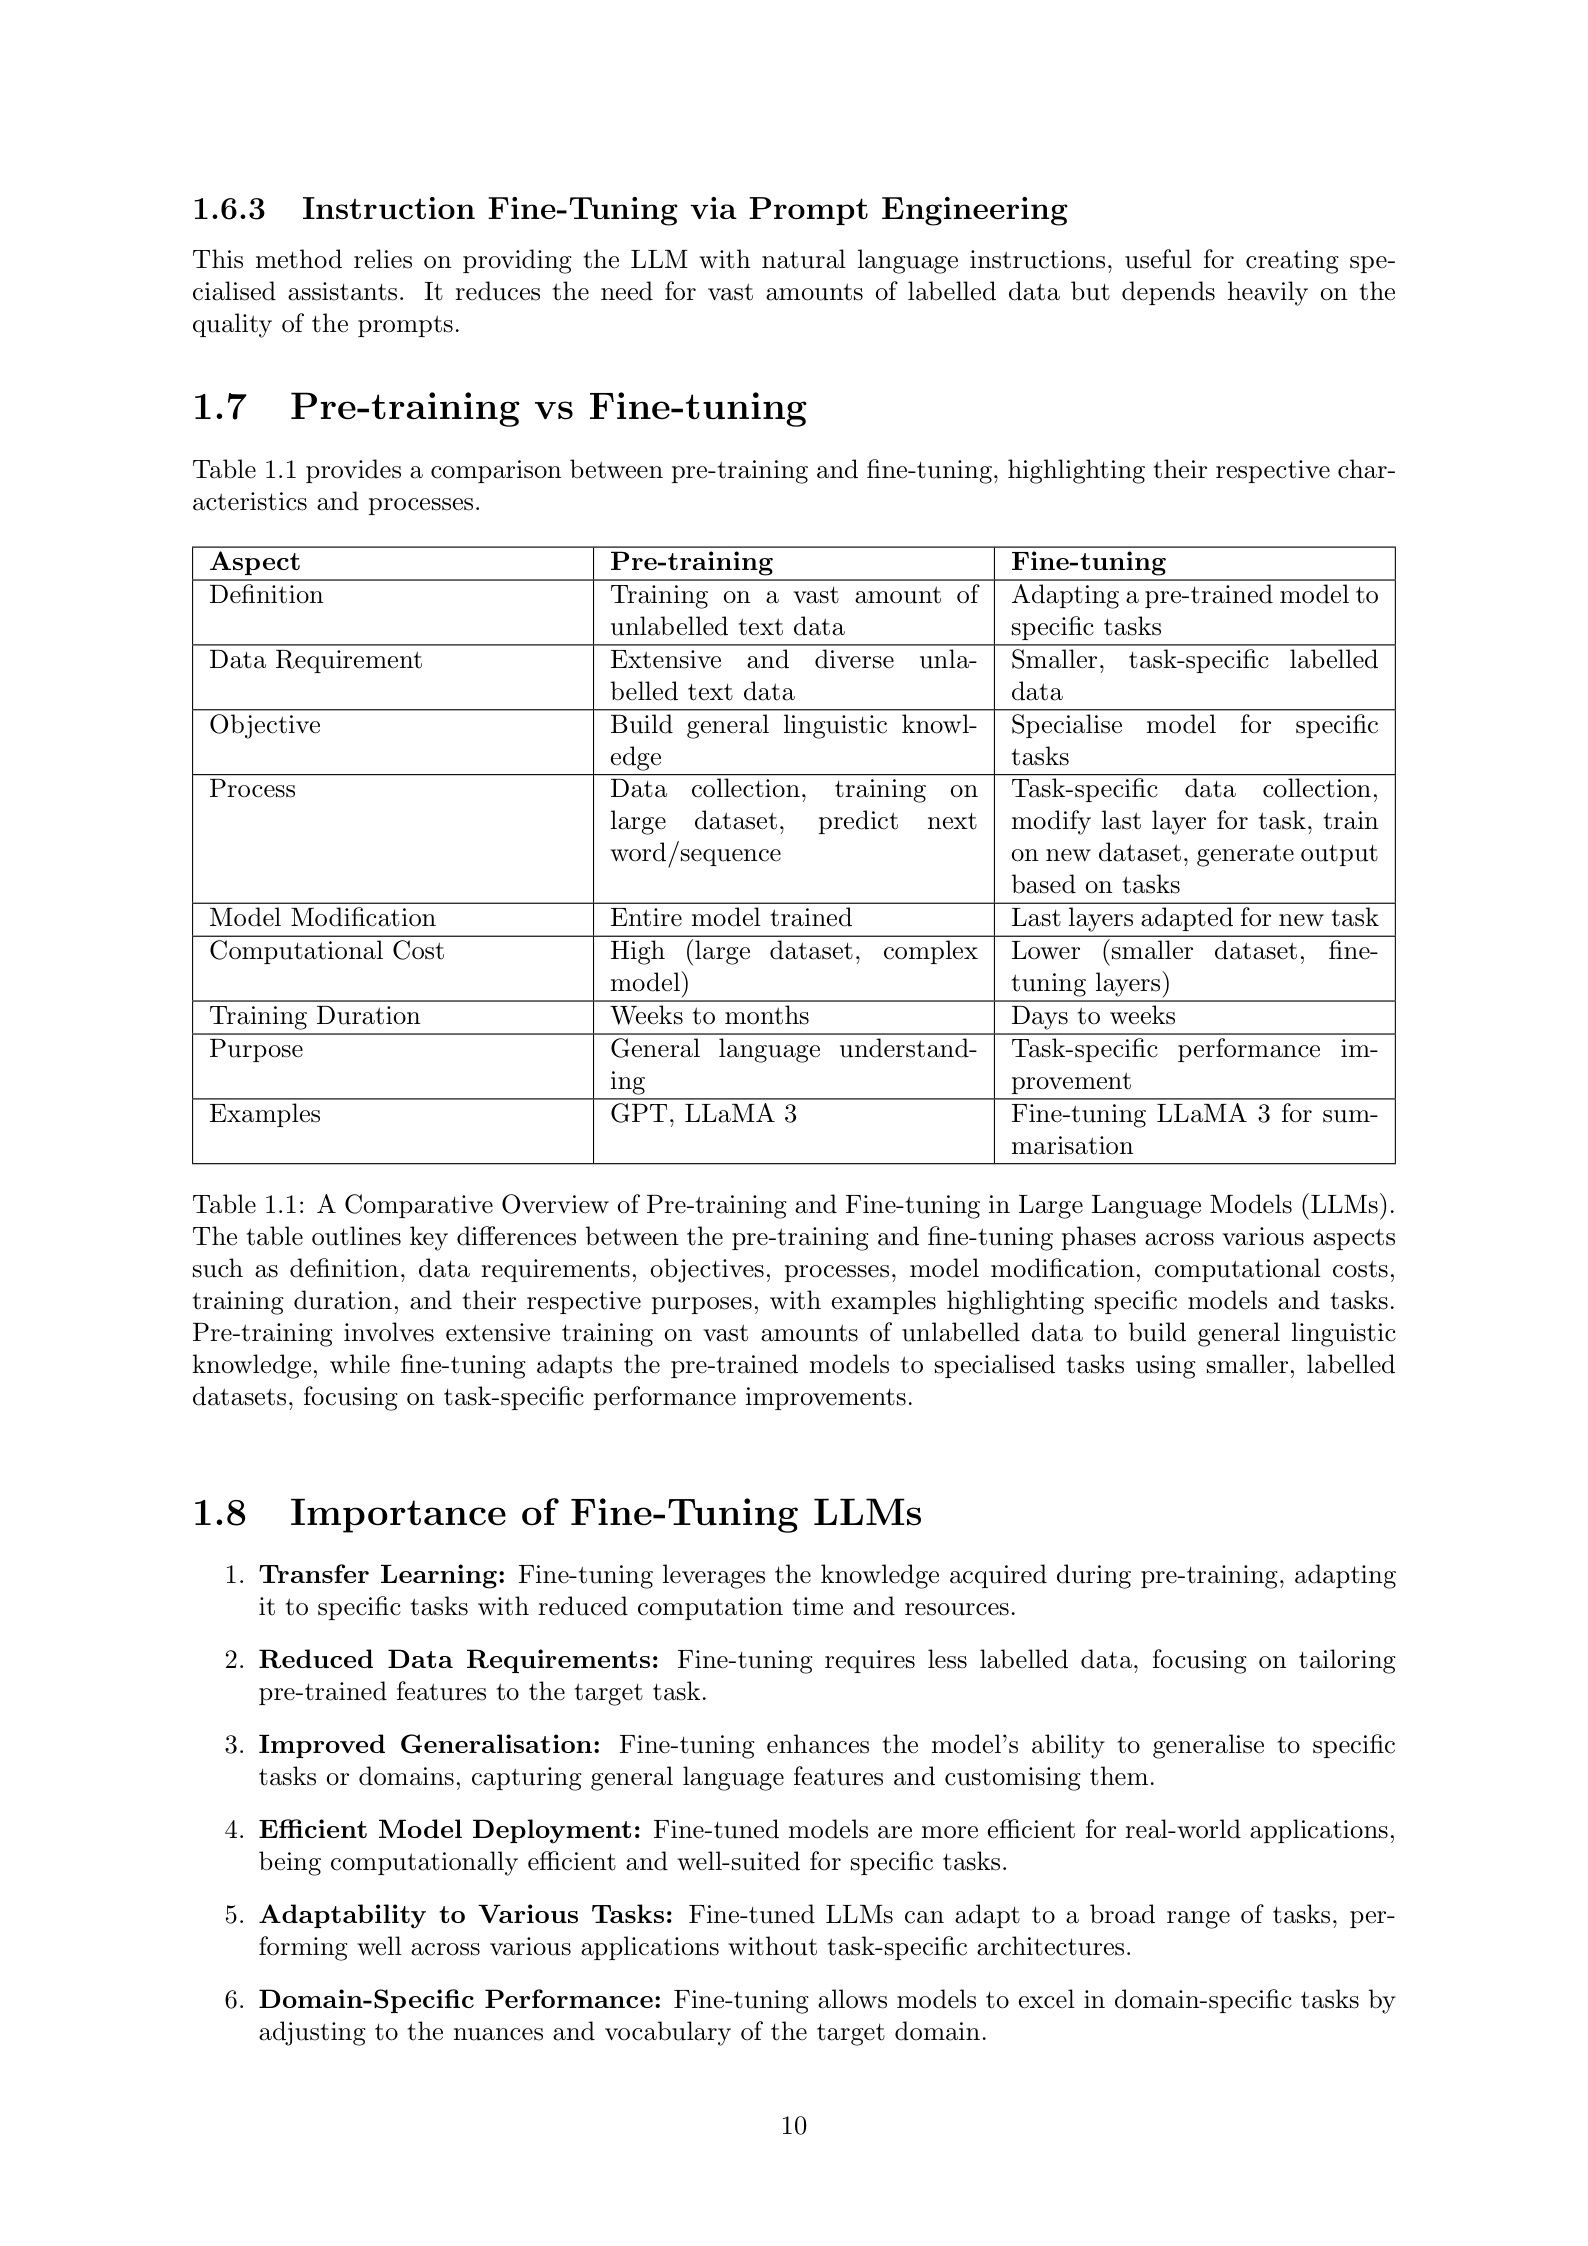
\includegraphics[width=\linewidth]{ocr_page12_original.png}
    \caption{Source page}
  \end{subfigure}\hfill
  \begin{subfigure}[t]{0.25\textwidth}
    \centering
    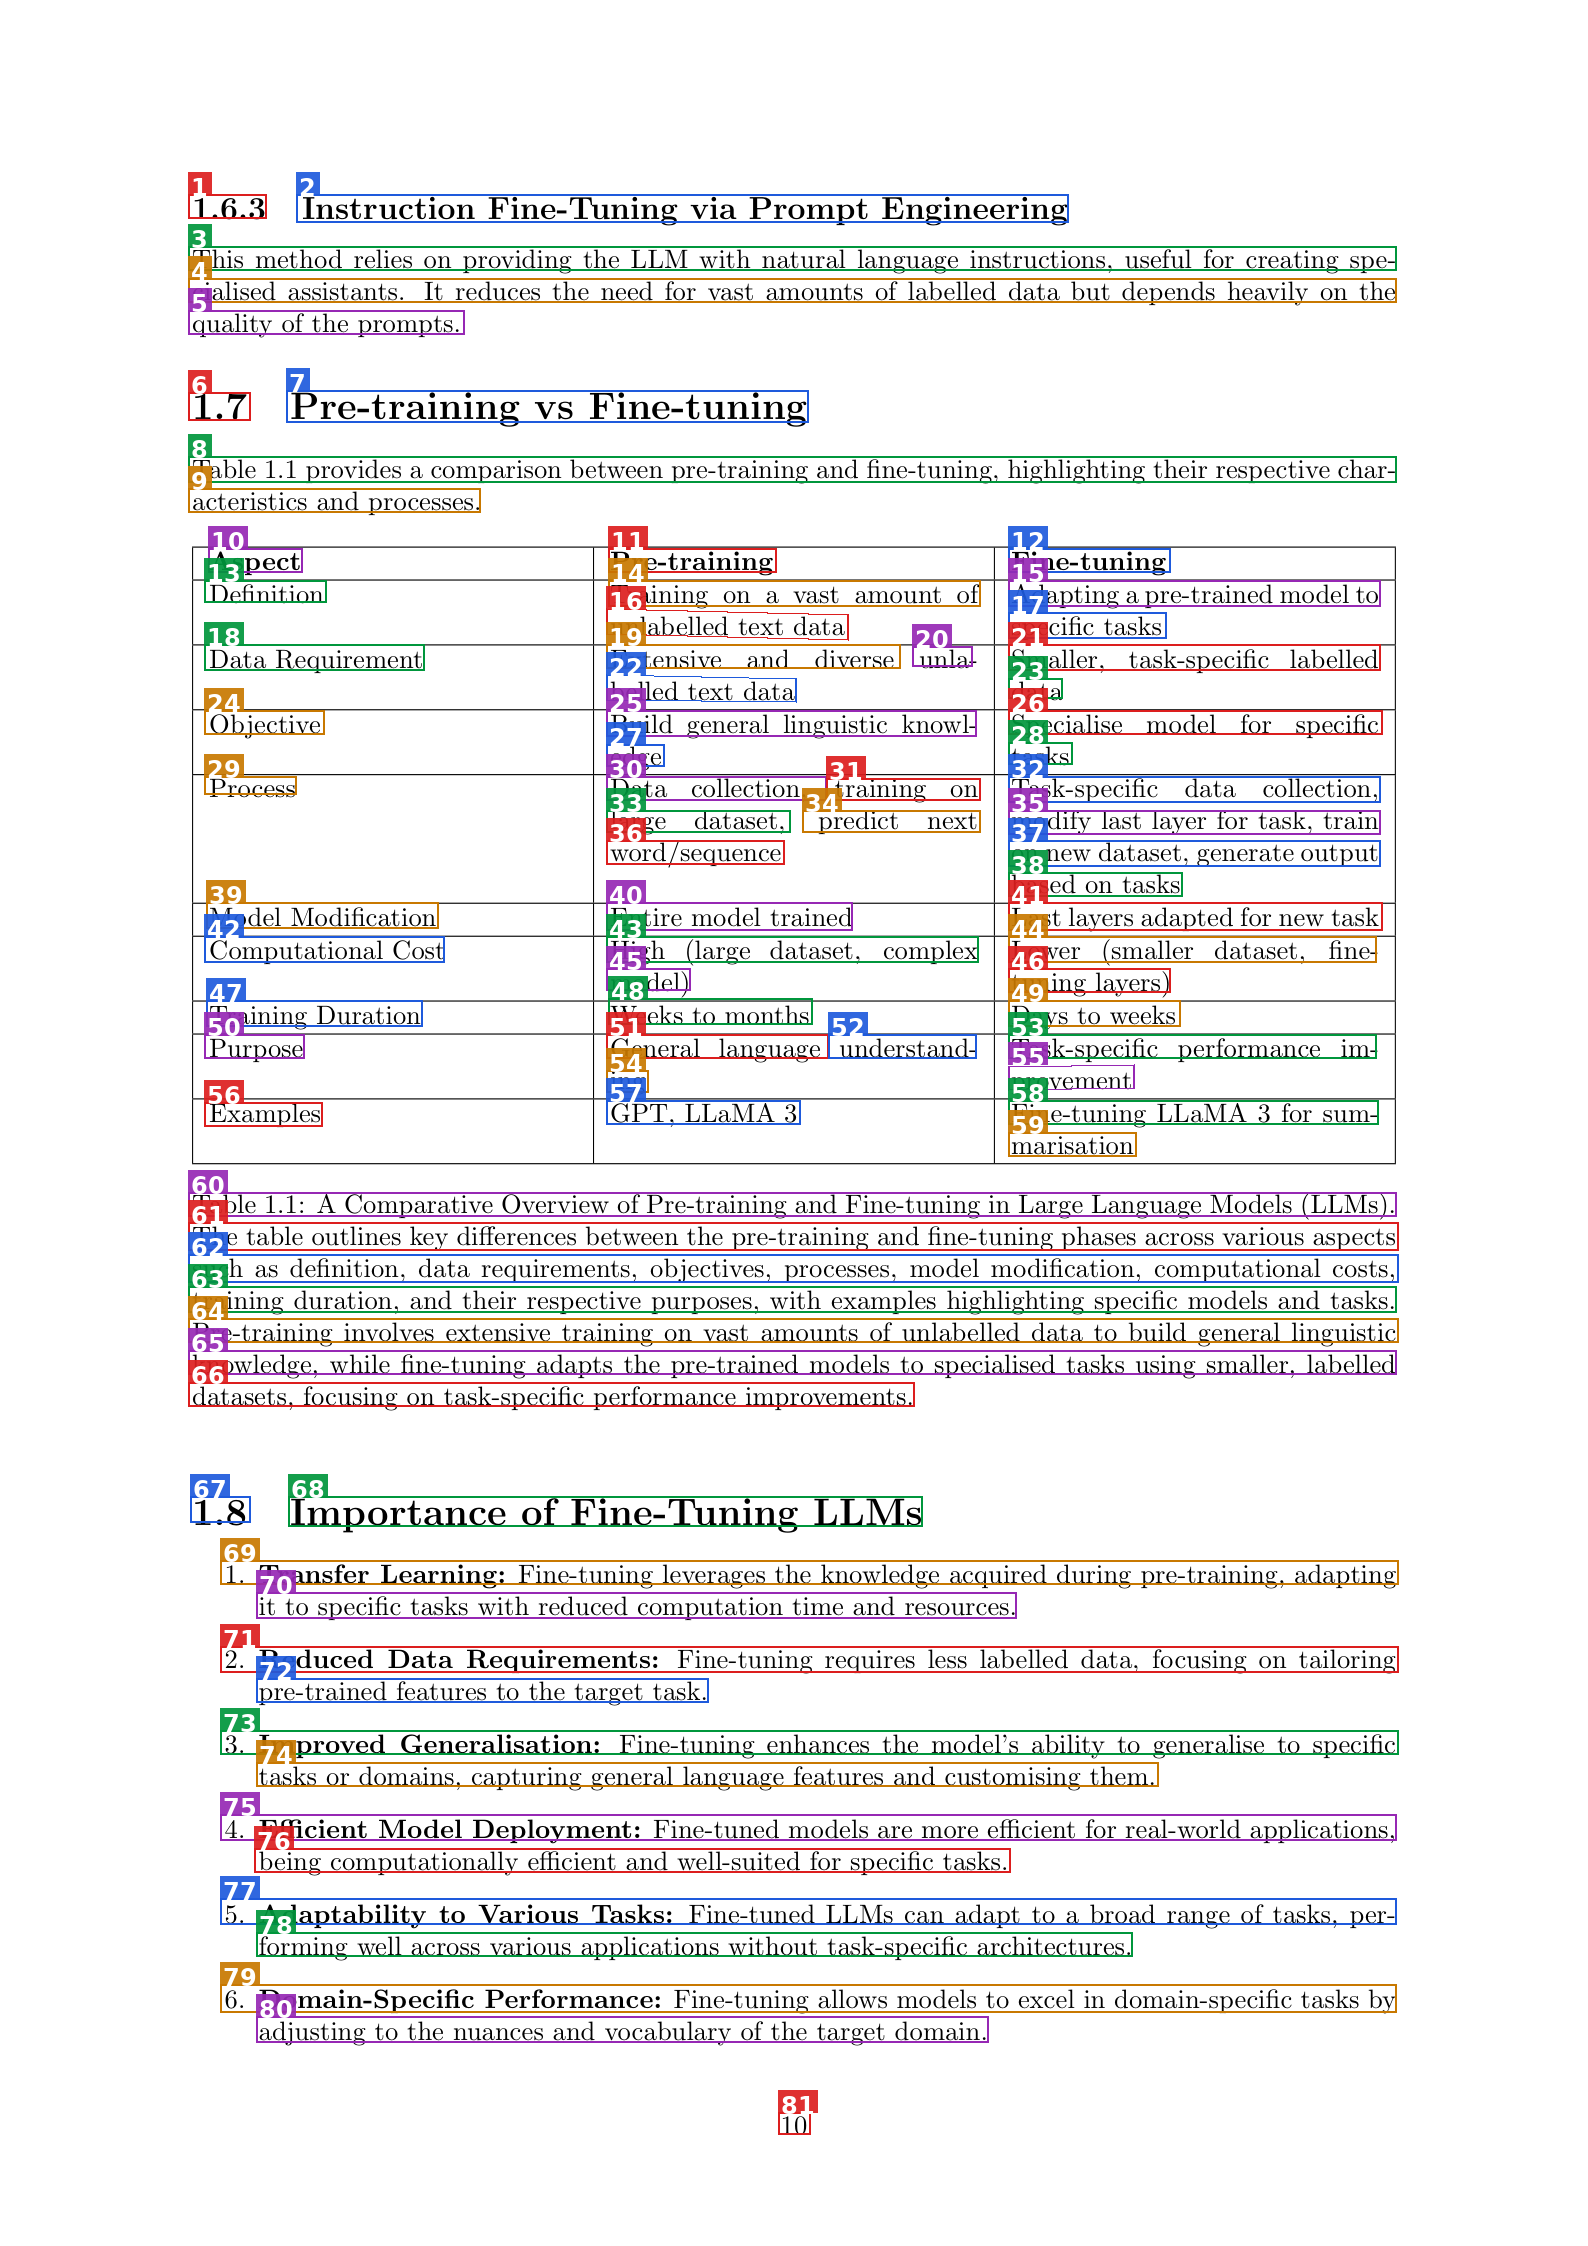
\includegraphics[width=\linewidth]{ocr_page12_detection.png}
    \caption{Text detection}
  \end{subfigure}\hfill
  \begin{subfigure}[t]{0.25\textwidth}
    \centering
    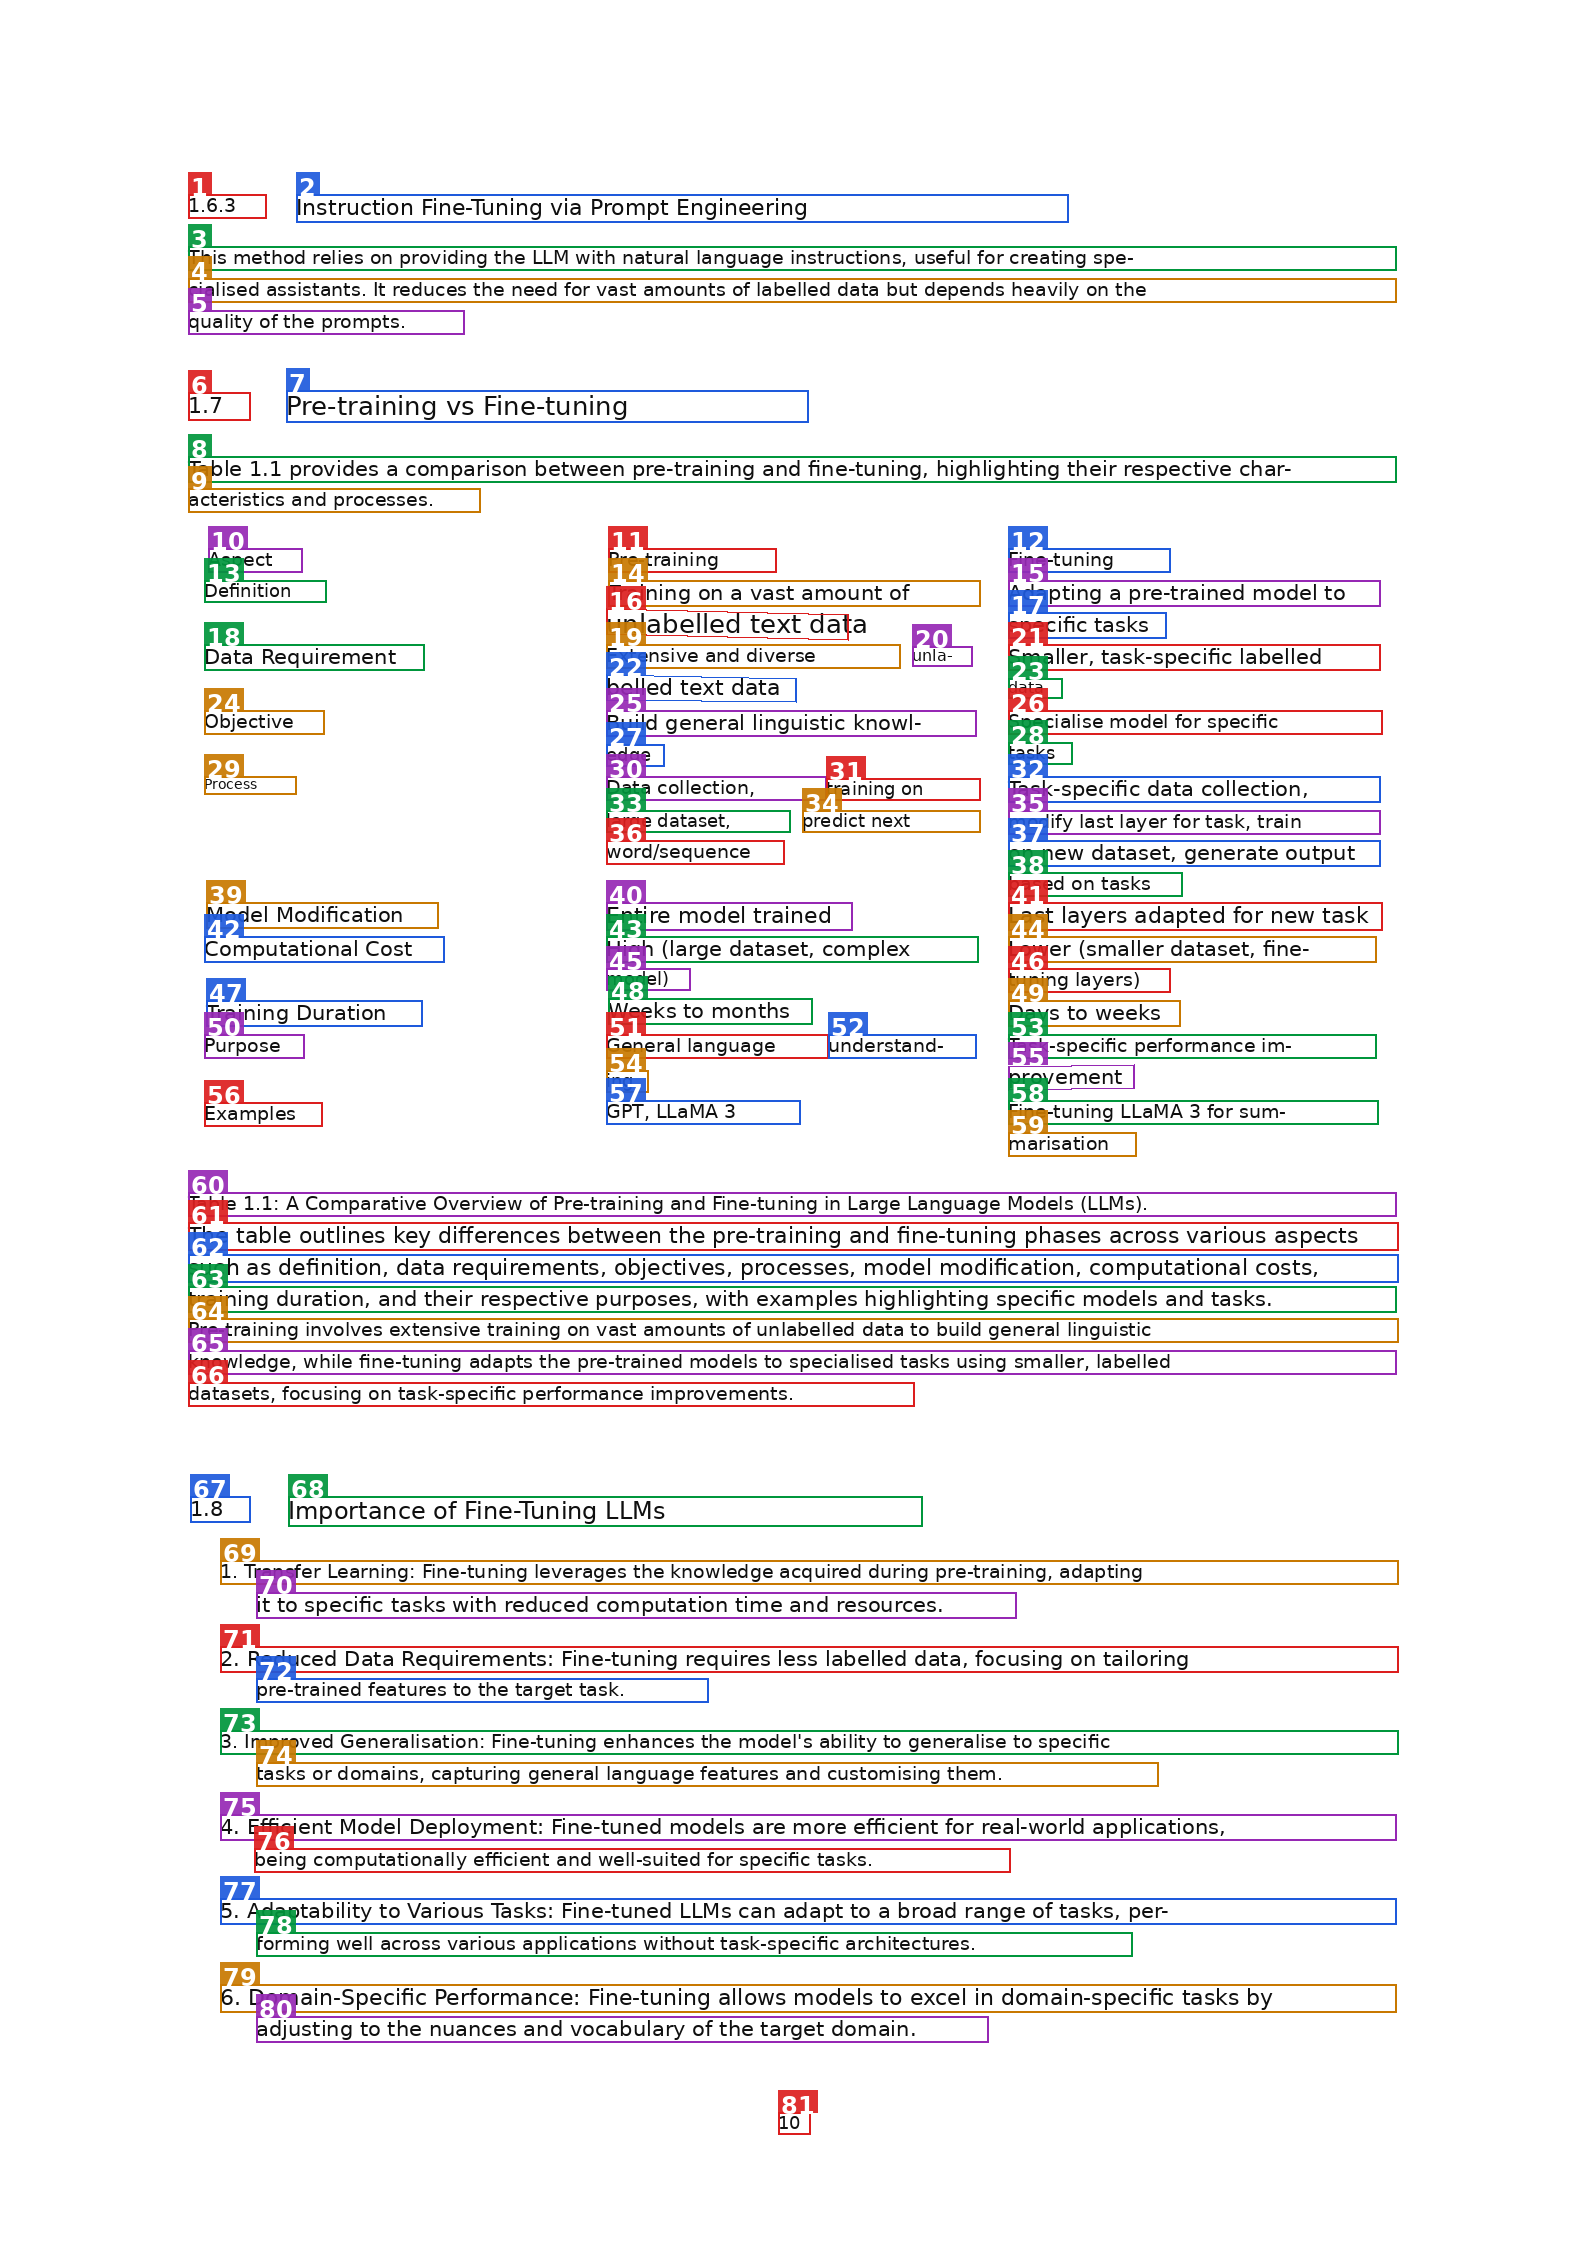
\includegraphics[width=\linewidth]{ocr_page12_recognition.png}
    \caption{Text recognition}
  \end{subfigure}\hfill
  \begin{subfigure}[t]{0.25\textwidth}
    \centering
    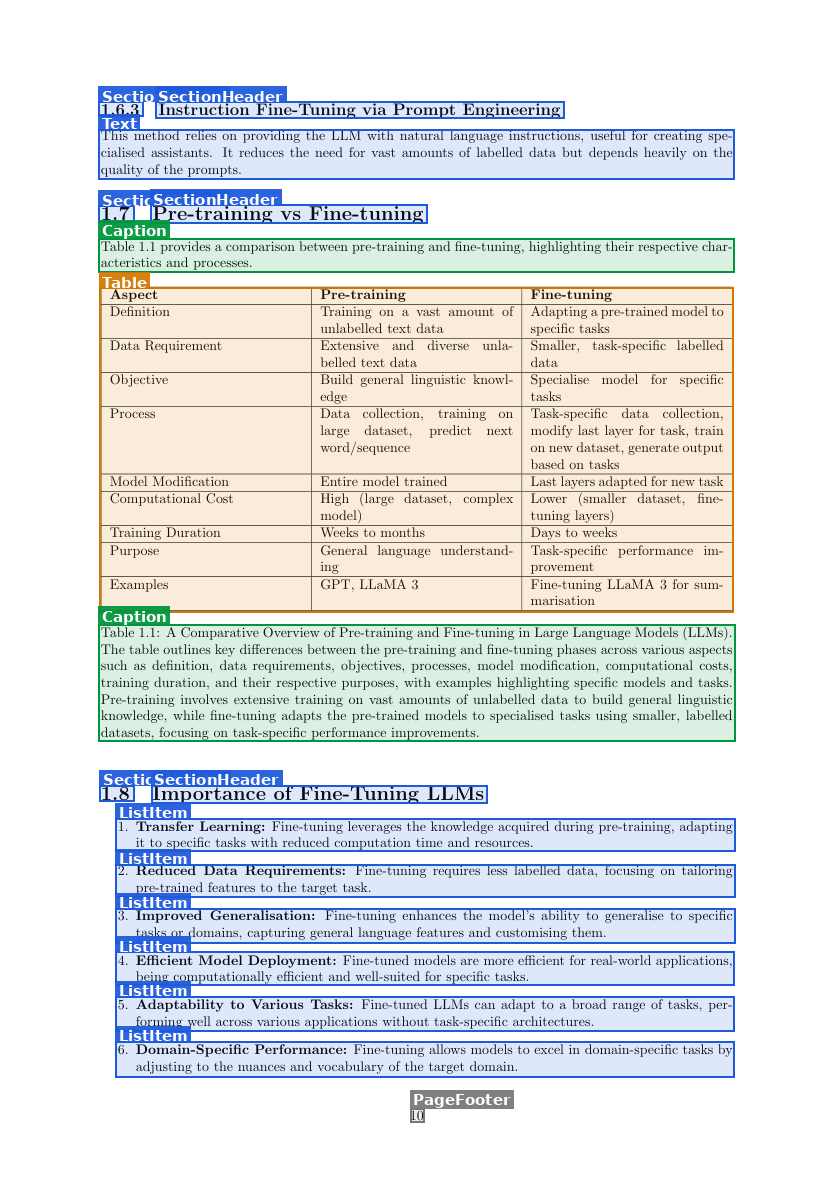
\includegraphics[width=\linewidth]{layout_page12.png}
    \caption{Layout detection}
  \end{subfigure}
  \caption{Page-level recognition stages: (a) the rasterised page is the input;
  (b) individual text lines are localised; (c) each line is recognised and
  re-anchored to its position; (d) the layout model delimits blocks, coloured by
  coarse \texttt{category} and labelled with the fine-grained class.}
  \label{fig:parser-stages}
\end{figure}

\begin{figure}[H]
  \centering
  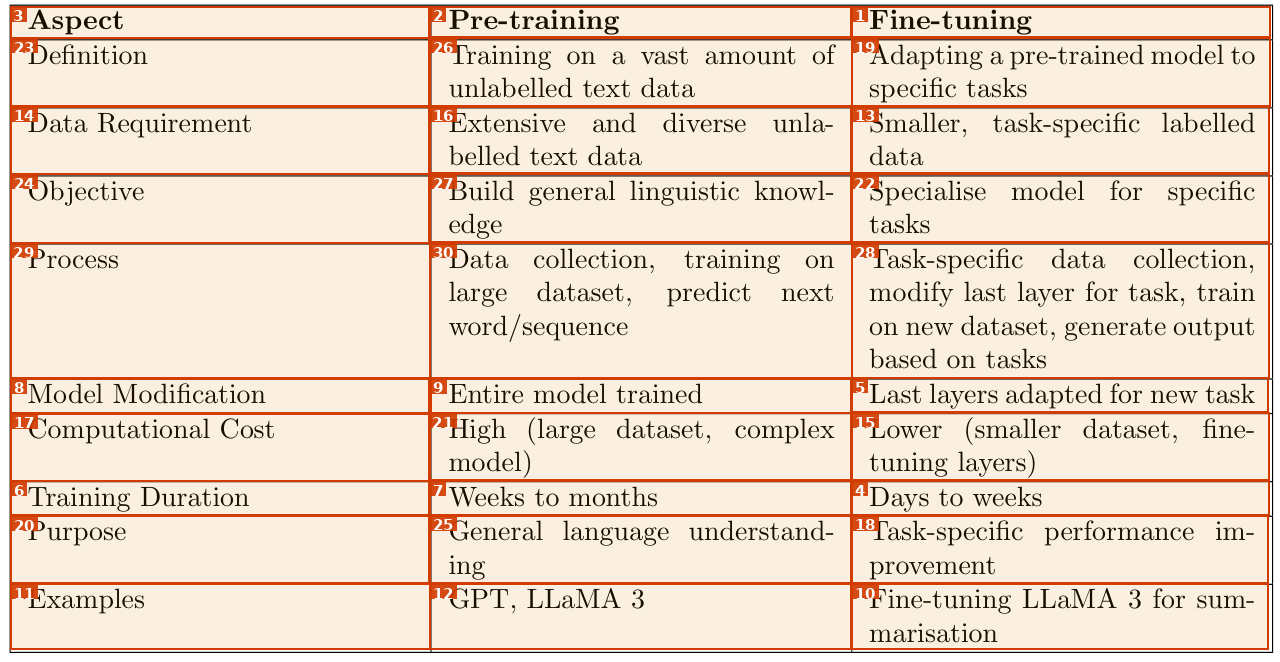
\includegraphics[width=0.4\linewidth]{table_cells_page12.png}
  \caption{Table-cell detection: the PaddleOCR RT-DETR detector returns a box per
  cell inside each table region; the boxes are kept as geometry for cell-wise
  translation and table reconstruction.}
  \label{fig:table-cells}
\end{figure}

The resulting \texttt{ParsedDocument} is a tree of pages and elements. Each
\texttt{ElementData} stores the fine label, coarse category, PDF-space bounding
box and source text. Table elements additionally store a flat list of cells,
each with a grid box and a tight text box. The fine labels are mapped to four
translation policies:

\begin{itemize}[leftmargin=1.2em]
  \item \texttt{FLOWING\_TEXT}: paragraphs, lists, captions, footnotes, section
  headers, forms and tables of contents; translated as text and re-wrapped.
  \item \texttt{TABLE}: translated cell by cell so content remains tied to its
  original cell geometry.
  \item \texttt{EQUATION}: isolated formula regions; preserved or processed by
  the formula-specific path.
  \item \texttt{BYPASS}: figures, pictures, code, page headers and footers;
  copied from the source page without translation.
\end{itemize}

\subsubsection{Translation-Oriented Post-processing}

Detected OCR lines are assigned to a layout block when at least $50\%$ of the
line area lies inside it, then sorted by row and $x$ position. Text is normalised
to NFC, control characters are removed except newline and tab, whitespace is
collapsed, and empty outer lines are trimmed.

Three repairs make the output useful for translation rather than plain
extraction. \texttt{BYPASS} blocks are kept as image regions. Sparse blocks are
split when formula regions contain multiple OCR lines or when wide intra-row
gaps reveal unrelated text clusters (Figure~\ref{fig:sparse-split}). Reading
order is repaired by expanding boxes over overlapping OCR lines (coverage
$\ge0.3$), pruning nested duplicates (containment $\ge0.7$) and promoting
unassigned OCR lines to \texttt{Text} (Figure~\ref{fig:reading-order}). These
steps never invent content; they
only attach existing OCR lines to geometric elements before translation.

\begin{figure}[H]
  \centering
  \begin{subfigure}[t]{0.47\textwidth}
    \centering
    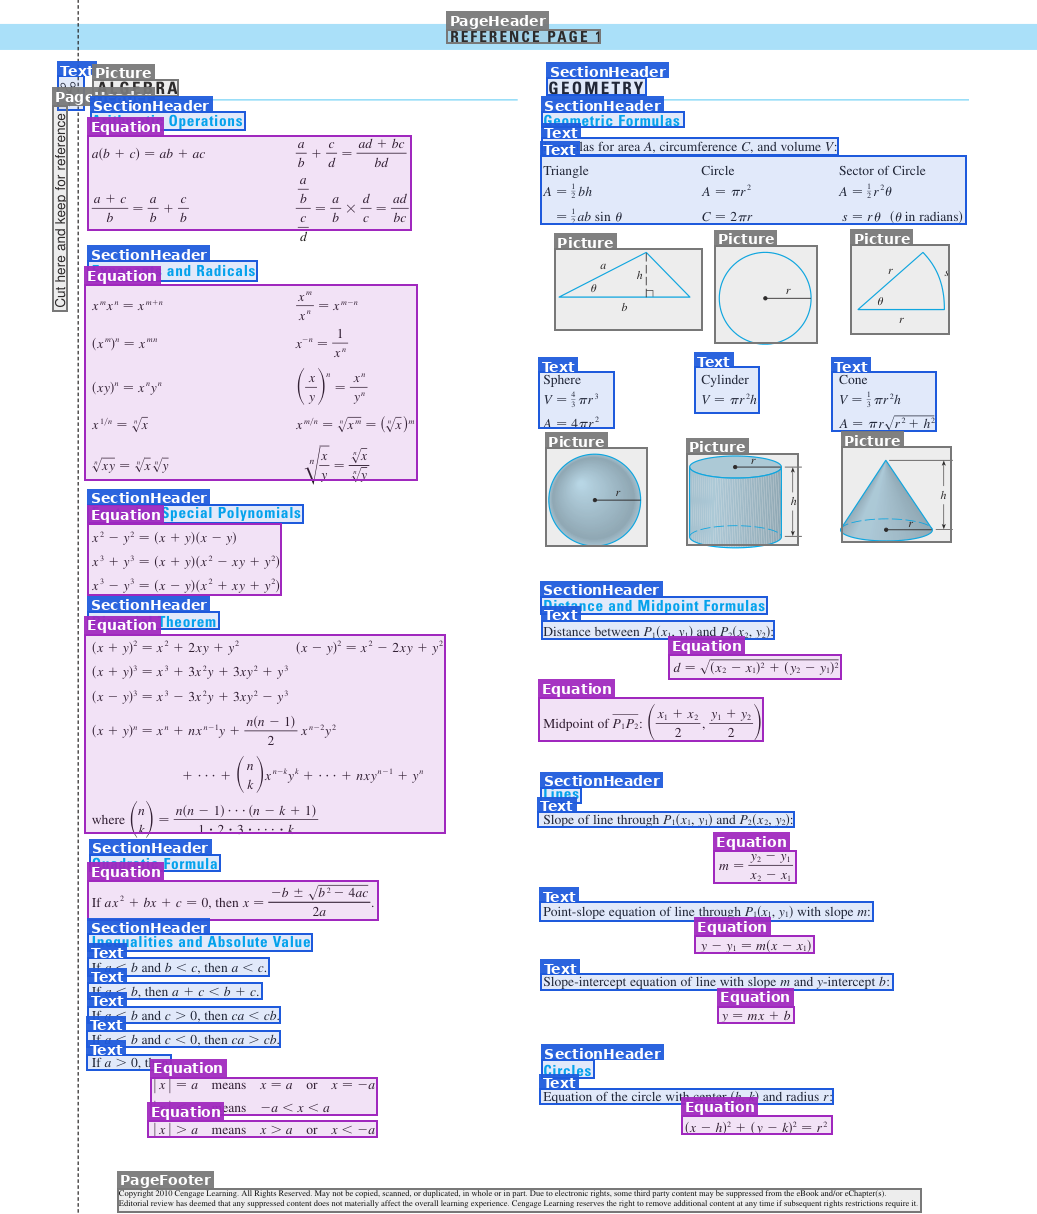
\includegraphics[width=0.8\linewidth]{layout_calculus_p2_before.png}
    \caption{Before splitting}
  \end{subfigure}\hfill
  \begin{subfigure}[t]{0.47\textwidth}
    \centering
    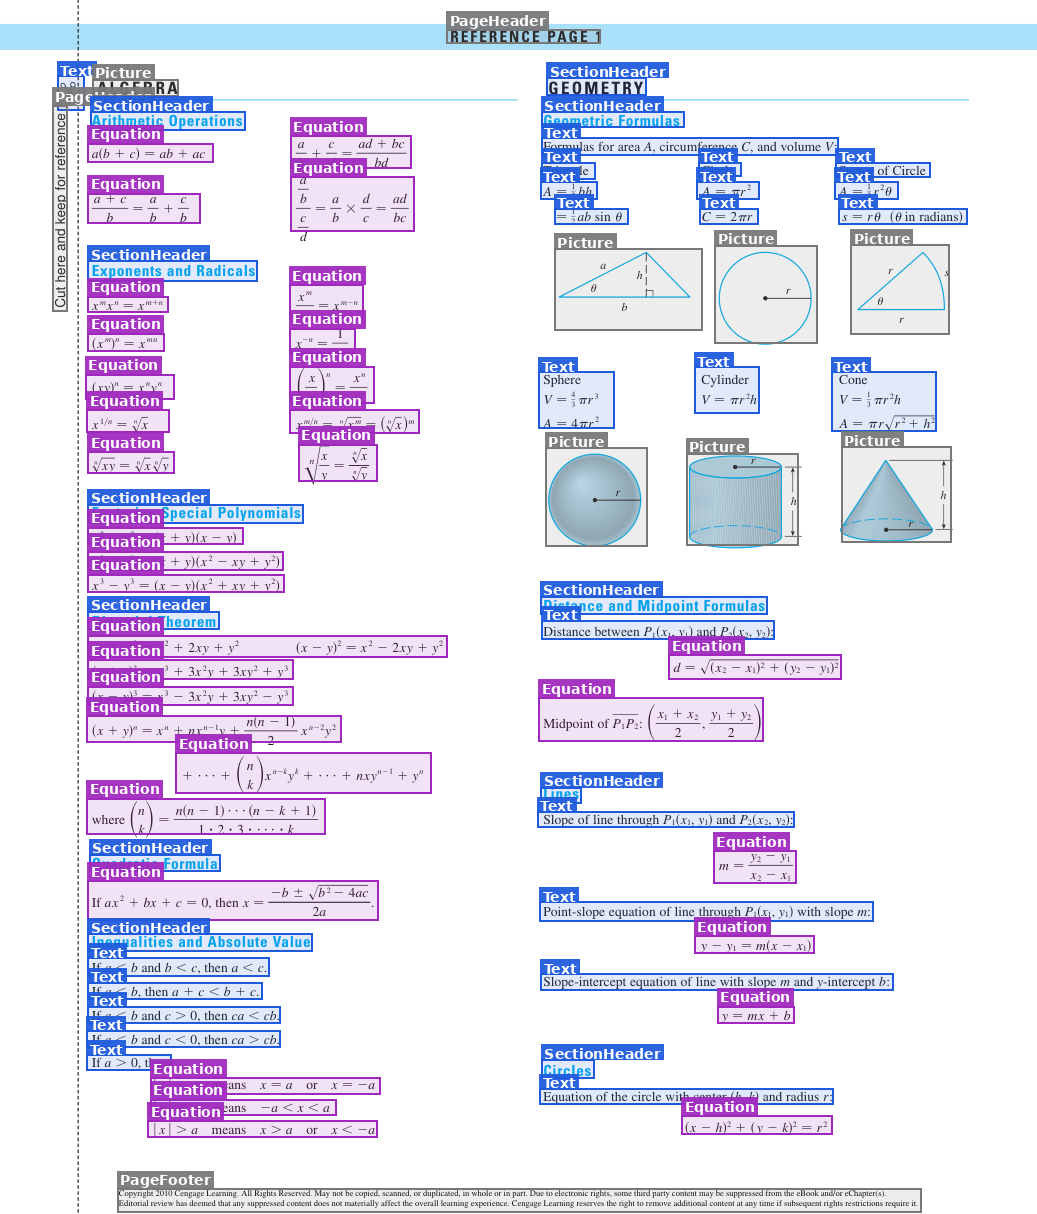
\includegraphics[width=0.8\linewidth]{layout_calculus_p2_after.png}
    \caption{After splitting}
  \end{subfigure}
  \caption{Sparse-block splitting separates formula-heavy regions into
  translatable line-level elements while preserving bypassed regions.}
  \label{fig:sparse-split}
\end{figure}

\begin{figure}[H]
  \centering
  \tikzset{
    blk/.style={draw, line width=0.6pt},
    tline/.style={draw=gray!55, fill=gray!22, line width=0.2pt},
    hot/.style={draw=red!80, fill=red!10, line width=0.5pt, dashed},
    hoton/.style={draw=red!80, fill=red!12, line width=0.5pt},
    ghost/.style={draw=gray!55, line width=0.5pt, dashed},
    lbl/.style={font=\scriptsize},
    tag/.style={font=\tiny\itshape, gray!55!black},
    num/.style={font=\scriptsize\bfseries, fill=white, inner sep=1pt},
    flow/.style={-{Latex}, line width=0.7pt},
  }
  \begin{subfigure}[t]{0.32\textwidth}\centering
  \begin{tikzpicture}[scale=0.85, transform shape]
    \draw[blk] (0,0) rectangle (2.2,1.4);
    \fill[tline] (0.2,1.02) rectangle (2.0,1.22);
    \fill[tline] (0.2,0.60) rectangle (2.0,0.80);
    \draw[hot]   (0.2,-0.22) rectangle (2.0,0.10);
    \node[tag] at (1.1,-0.5) {tight box, line spills};
    \draw[flow] (2.55,0.5) -- (3.25,0.5) node[midway,above,font=\tiny]{$\ge0.3$};
    \begin{scope}[xshift=3.6cm]
      \draw[blk] (0,-0.30) rectangle (2.2,1.4);
      \fill[tline] (0.2,1.02) rectangle (2.0,1.22);
      \fill[tline] (0.2,0.60) rectangle (2.0,0.80);
      \fill[hoton] (0.2,-0.18) rectangle (2.0,0.14);
      \node[tag] at (1.1,-0.55) {box hugs glyphs};
    \end{scope}
  \end{tikzpicture}
  \caption{Boundary expansion}
  \end{subfigure}\hfill
  \begin{subfigure}[t]{0.32\textwidth}\centering
  \begin{tikzpicture}[scale=0.85, transform shape]
    \draw[blk] (0,0.15) rectangle (2.2,1.4);
    \draw[hot] (0.28,0.42) rectangle (1.5,1.15);
    \draw[blk] (0,-0.95) rectangle (2.2,-0.15);
    \node[tag] at (1.1,-1.3) {contained in larger};
    \draw[flow] (2.55,0.2) -- (3.25,0.2) node[midway,above,font=\tiny]{$\ge0.7$};
    \begin{scope}[xshift=3.6cm]
      \draw[blk] (0,0.15) rectangle (2.2,1.4);
      \draw[ghost] (0.28,0.42) rectangle (1.5,1.15);
      \draw[red!80, line width=0.5pt] (0.28,0.42)--(1.5,1.15) (0.28,1.15)--(1.5,0.42);
      \draw[blk] (0,-0.95) rectangle (2.2,-0.15);
      \node[num] at (0.32,1.08) {1};
      \node[num] at (0.32,-0.55) {2};
      \node[tag] at (1.1,-1.3) {pruned, re-sorted};
    \end{scope}
  \end{tikzpicture}
  \caption{Containment pruning}
  \end{subfigure}\hfill
  \begin{subfigure}[t]{0.32\textwidth}\centering
  \begin{tikzpicture}[scale=0.85, transform shape]
    \draw[blk] (0,0.75) rectangle (2.2,1.45);
    \node[num] at (0.32,1.10) {1};
    \draw[hot] (0.2,0.28) rectangle (2.0,0.56);
    \node[tag, red!70!black] at (1.1,0.1) {orphan (no block)};
    \draw[blk] (0,-0.85) rectangle (2.2,-0.35);
    \node[num] at (0.32,-0.60) {2};
    \draw[flow] (2.55,0.4) -- (3.25,0.4) node[midway,above,font=\tiny]{promote};
    \begin{scope}[xshift=3.6cm]
      \draw[blk] (0,0.75) rectangle (2.2,1.45);
      \node[num] at (0.32,1.10) {1};
      \draw[blk] (0,0.20) rectangle (2.2,0.62);
      \node[num] at (0.32,0.41) {2};
      \node[lbl] at (1.35,0.41) {\texttt{Text}};
      \draw[blk] (0,-0.85) rectangle (2.2,-0.35);
      \node[num] at (0.32,-0.60) {3};
      \node[tag] at (1.1,-1.15) {inserted in order};
    \end{scope}
  \end{tikzpicture}
  \caption{Orphan-line insertion}
  \end{subfigure}
  \caption{Reading-order repair (before $\rightarrow$ after; solid black = layout
  block, grey = OCR text line, red dashed = affected element). (a) OCR lines
  overlapping a block by at least $0.3$ are absorbed and the block expands to hug
  the glyphs. (b) A block is removed when $\ge 0.7$ of its area lies inside a
  larger retained block, and the rest are re-sorted by position. (c) An OCR line
  covered by no block becomes a \texttt{Text} element inserted at the right
  position in the reading sequence.}
  \label{fig:reading-order}
\end{figure}

For tables, the parser keeps detected cells as a flat coordinate list rather
than inferring a full HTML tree. This is enough
for cell-wise translation and
grid reconstruction while avoiding brittle table-structure inference. Pages are
rasterised at two resolutions: a standard resolution for layout and detection,
and a higher one for text recognition, which is the part most sensitive to small
or blurred glyphs.

\subsection{Stage 2: Content Translation}
\label{subsec:method-translate}

This stage translates the source text of the \texttt{ParsedDocument}. Its main
task is preserving the link between content and geometry across model calls:
every translated string must return to the element or cell it came from, and
non-textual structure must stay addressable.

\subsubsection{Translation Units and Prompt Contract}
\label{subsubsec:prompt}

Each translatable element becomes one unit; table cells become separate units;
formula blocks are routed through the path in Section~\ref{subsubsec:special}.
Units are packed into bounded chunks in document order, giving the model local
context while keeping responses small enough to validate.

The central contract is an identifier bijection: every input unit identifier
must appear exactly once in the model output. The prompt also injects
document-level glossary entries relevant to the chunk, preserves URLs,
placeholders, tags and mathematical expressions, requests Typst-compatible math
inside \texttt{<math>...</math>}, and states the $\pm15\%$ character-length
preference evaluated later. Semantic adequacy is prioritised above that length
preference.

Outputs are accepted only after identifier and content validation. If the
identifier contract fails, only the affected units are requested again; if
repair still fails, the source string is kept and the event is logged so no
region is left empty in the final PDF.

\subsubsection{Handling Tables and Formulas}
\label{subsubsec:special}

Tables and formulas bypass the ordinary text path. For tables, the dominant risk
is OCR corruption: a single wrong digit or symbol can invalidate a row. Before
translation, the system crops the table from the source page and asks a
multimodal model to verify the per-cell OCR; returned corrections overwrite the
OCR data before cell-wise translation.

For formulas, the difficult case is a block that mixes prose and notation. Pure
formula regions are skipped; mixed regions are cropped and sent to a vision
model that translates the prose while preserving the mathematics, wrapped in the
\texttt{<math>} syntax required by reconstruction.

\subsubsection{Format Post-processing}

After all segments are translated, two cross-segment structures are repaired.
Tables of contents are reshaped into \verb|"<title>\t<page>"| lines when
per-line translation collapses dot leaders. Residual formulas in ordinary text
are detected from LaTeX commands, Greek symbols and super/subscript syntax, then
re-wrapped or converted to valid \texttt{<math>} Typst syntax. Invalid repairs
are rejected and the previous renderable translation is kept.

\subsection{Stage 3: Document Reconstruction}
\label{subsec:method-render}

Reconstruction is where H2 is enforced. The translator has strings but not the
page: it cannot know which neighbour a block would collide with, which font size
preserves the page hierarchy, or what colour should cover and replace the source
glyphs. The reconstruction stage therefore owns geometry and appearance.

\subsubsection{Size Selection}
\label{subsubsec:sizing}

For a text string and a box, the primitive operation is \texttt{autofit}: binary
search for the largest font size whose wrapped text fits the box height. The
pipeline does not simply use that value on each translated block. Instead, it
groups same-role elements, computes \texttt{autofit} on their \emph{source} text,
clusters the source sizes in one dimension, and uses the cluster median as the
canonical size for that role. This preserves the source document's typographic
hierarchy.

Translated text departs from the canonical size only when necessary
(Figure~\ref{fig:overflow-collision}). If it fits, the canonical size is kept.
If it overflows into local free space, the canonical size is still kept and only
the typesetting frame is extended. A block is shrunk toward its translated
\texttt{autofit} only when the overflow intersects a neighbouring retained
element. The experiments use fixed parameters for clustering, the 7~pt
readability floor, the 80~pt expansion cap and the table-cell scale factor
(Appendix~\ref{app:implementation}).

\begin{figure}[H]
    \centering
    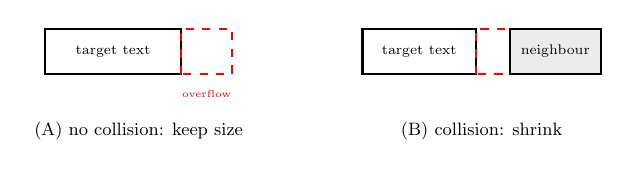
\begin{tikzpicture}[scale=0.72, transform shape]
        \begin{scope}
            \draw[thick] (0,0) rectangle (2.4,0.8);
            \node[font=\scriptsize] at (1.2,0.4) {target text};
            \draw[dashed, thick, red] (2.4,0) rectangle (3.3,0.8);
            \node[font=\tiny, red] at (2.85,-0.35) {overflow};
            \node[font=\small] at (1.65,-1.0) {(A) no collision: keep size};
        \end{scope}
        \begin{scope}[xshift=5.6cm]
            \draw[thick] (0,0) rectangle (2.0,0.8);
            \node[font=\scriptsize] at (1.0,0.4) {target text};
            \draw[dashed, thick, red] (2.0,0) rectangle (2.9,0.8);
            \draw[thick, fill=gray!15] (2.6,0) rectangle (4.2,0.8);
            \node[font=\scriptsize] at (3.4,0.4) {neighbour};
            \node[font=\small] at (2.1,-1.0) {(B) collision: shrink};
        \end{scope}
    \end{tikzpicture}
    \vspace{0.4em}
    \caption{Font size changes only when rendered overflow would collide with a
    neighbouring element.}
    \label{fig:overflow-collision}
\end{figure}

\subsubsection{Colour Selection}
\label{subsubsec:colour}

Two colours must be inferred for each translated element: the background used to
mask the source text and the colour used to draw the target text. Neither is
available uniformly from the PDF content stream, so both are sampled from the
rendered page (Figure~\ref{fig:colour-sampling}). Background colour comes from a
6~pt ring around the element at $2\times$ raster scale; contaminated light rings
are trimmed before taking a per-channel median. Text colour comes from the
central $60\%$ of the box: pixels whose RGB distance from the background exceeds
80 are glyph candidates, and the foreground is the median of the furthest half.
The rule is orientation-free, so it works for dark-on-light, light-on-dark and
saturated slide text. Textured backgrounds and boxes whose centre is mostly
whitespace remain expected failure cases.

\begin{figure}[H]
    \centering
    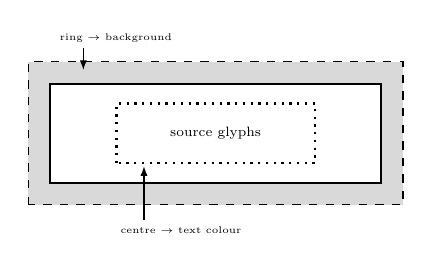
\begin{tikzpicture}[scale=0.7, transform shape]
        \fill[gray!30] (-0.4,-0.4) rectangle (6.4,2.2);
        \fill[white]   (0,0)       rectangle (6,1.8);
        \draw[dashed]  (-0.4,-0.4) rectangle (6.4,2.2);
        \draw[thick]   (0,0)       rectangle (6,1.8);
        \draw[dotted, thick] (1.2,0.36) rectangle (4.8,1.44);
        \node[font=\scriptsize] at (3,0.9) {source glyphs};
        \node[font=\tiny, anchor=west] at (0.05,2.62)
              {ring $\rightarrow$ background};
        \node[font=\tiny, anchor=west] at (1.15,-0.85)
              {centre $\rightarrow$ text colour};
        \draw[-{Latex[length=1.2mm]}] (0.6,2.45) -- (0.6,2.05);
        \draw[-{Latex[length=1.2mm]}] (1.7,-0.68) -- (1.7,0.30);
    \end{tikzpicture}
    \caption{Background is sampled around the element; text colour is sampled
    from pixels far from that background inside the box.}
    \label{fig:colour-sampling}
\end{figure}

The background estimate is used for both the overlay rectangle and, on
born-digital pages, the redaction that removes native source glyphs while
preserving images and line art. Font style is chosen by element role, and an
ordered fallback chain lets the typesetter resolve Vietnamese diacritics and CJK
ideographs per character.

\subsubsection{Overlay Compilation and Output}
\label{subsubsec:overlay}

The overlay is compiled with Typst~\citep{typst}, chosen for multilingual text
and mathematical syntax. Each translated element contributes a background
rectangle and target text at the selected position, size and colour. The overlay
is then composited page by page over the source PDF; untranslated figures,
charts and \texttt{BYPASS} regions remain from the original document. The result
is compressed and cleaned before being returned.

\subsection{Experimental Design}
\label{subsec:method-eval}

The experiments test H1 and H2 at two levels. Translation is measured on
WMT24++ (M2, M3), structure analysis on OmniDocBench and PubTables-1M (M1), and
complete translated PDFs on a shared DocLayNet-derived corpus. The latter
uses the same source pages, target language and output-level metrics for every
system, treating each pipeline as a black box.

\subsubsection{Translation Quality}
\label{subsubsec:eval-mt}

We use all 55 \texttt{en}$\rightarrow$\texttt{xx} WMT24++ pairs
(\citealp{wmt24pp}); after filtering rows flagged \texttt{is\_bad\_source},
each system translates 52{,}800 segments. Five models are compared with all
non-model settings fixed:
\texttt{\seqsplit{gemini-2.5-flash-lite}},
\texttt{\seqsplit{gemini-3.1-flash-lite}},
\texttt{\seqsplit{gpt-4.1-nano}}, \texttt{\seqsplit{gpt-5.4-nano}} and
\texttt{\seqsplit{qwen/qwen3.5-flash-02-23}}.

COMET-DA (\texttt{Unbabel/wmt22-comet-da}) is the primary adequacy metric because
it scores the source, hypothesis and reference jointly and correlates better
with human judgement than surface-overlap metrics~\citep{comet,wmt-metrics-shared-task}.
chrF++~\citep{chrf}, computed with \texttt{sacrebleu}, is reported as a lexical
diagnostic. We also record median seconds per document and source words per
second. For the length constraint, a segment complies when
$|\text{len}_{\text{tgt}}/\text{len}_{\text{src}} - 1| \le 0.15$ in characters;
segments shorter than 20 characters are exempt.

\subsubsection{Structure Analysis Accuracy}
\label{subsubsec:eval-parser}

The parser is scored against OmniDocBench~\citep{omnidocbench}: 1{,}651 pages
with block boxes, labels, text, formulas, tables, reading order and slice
attributes such as language, layout and document source. Predictions and ground
truth are brought into a shared frame by normalising coordinates to
$[0,1]\times[0,1]$, reducing polygons to axis-aligned boxes, mapping labels into
coarse groups, discarding \texttt{abandon}/\texttt{other} blocks, and expanding
ground-truth \texttt{merge\_list} entries to the fine granularity used in
reporting.

The metric set is intentionally multi-view but compact (Table~\ref{tab:structure-metrics}).
Its distinctive point is that it separates \emph{coverage loss}, which the
translator cannot recover, from \emph{granularity differences}, which the
pipeline can often reassemble.

Localisation is the clearest example. We report both a strict COCO-style 1-1
matcher and a granularity-invariant $N$--$M$ matcher, with headline $F_1@.5$ and
mF1 averaged over thresholds $0.50,0.55,\dots,0.95$. The 1-1 matcher asks
whether one predicted box matches one annotated box. The $N$--$M$ matcher first
links predictions and ground truth into connected components when IoU or
intersection-over-area ($\mathrm{IoA}(A,B)=|A\cap B|/|A|$) is at least $0.5$,
then scores the union of each
component at the reporting threshold. Reading the pair of scores prevents a
translation-oriented split from being counted as pure detection loss.

For content-bearing metrics, predictions are paired to each ground-truth region
by union-gather: all predicted fragments whose area mostly lies inside the
region are collected, ordered and concatenated. This is essential because the
parser intentionally splits sparse blocks; matching only one fragment would
punish a translation-oriented design as if it had lost content.

The same pairing supplies different evidence to different tasks. The majority
coarse label in the gathered group gives classification accuracy; concatenated
normalised text gives OCR edit distance, CER and WER; the smallest emitted
element index gives the parser reading-order key. For formulas, edit distance is
reported but not treated as sufficient, because equivalent mathematical notation
can render identically while differing as strings. CDM is therefore included as
the formula-specific measure. For tables, OmniDocBench supplies a polygon and a
markup transcription per table but no per-cell boxes, so it can only support
whole-table coverage and text accuracy; cell geometry is measured on a second
corpus below. Logical structure---which cell spans which rows and columns---is
outside the scope of both, because the parser emits cell geometry only.

\begin{table}[H]
\centering
\caption{Structure-analysis metrics and the question each answers.}
\label{tab:structure-metrics}
\small
\setlength{\tabcolsep}{5pt}
\begin{tabularx}{\textwidth}{@{}l >{\raggedright\arraybackslash}X@{}}
\toprule
\textbf{Metric family} & \textbf{Purpose} \\
\midrule
Localisation & COCO 1-1 gives strict box matching; $N$--$M$ union matching gives
granularity-invariant region coverage. The gap is read as over/under-segmentation
cost rather than plain detection failure. \\
Classification & Coarse label accuracy on matched regions, separated from
class-agnostic localisation to avoid double penalties. \\
OCR & Normalised edit distance, CER and WER on matched text groups; CER is the
primary reading for CJK because WER depends on space-delimited words. \\
Reading order & Normalised edit distance between the annotated order and the
parser's emitted order over the same matched regions. \\
Formulas & Detection coverage, edit distance on matched/all formulas, and
CDM~\citep{cdm}, whose rendered-symbol comparison avoids penalising equivalent
LaTeX notation. \\
Tables & Whole-table content coverage and edit distance/CER on OmniDocBench.
Cell geometry is scored separately on PubTables-1M, whose annotations define a
cell as the intersection of its rows and columns and therefore include blank
cells. \\
\bottomrule
\end{tabularx}
\end{table}

\paragraph{Cell geometry.}
Cell-level localisation is evaluated separately on 1{,}499 cropped tables sampled
from the 93{,}834 tables in the PubTables-1M test split~\citep{pubtables1m}.
The subset is stratified by the presence of spanning cells ($52.7\%$) and by
cell count. PubTables-1M is chosen because its cell annotations correspond to
the intersections of table rows and columns, including blank cells, matching
the parser's output convention. Ground-truth cells are generated using the
dataset's reference implementation and matched one-to-one to predictions by
optimal IoU assignment. We report precision, recall, and $F_1$ at fixed IoU
thresholds and AP averaged over $0.50,0.55,\dots,0.95$. As the tables are
provided as crops, this evaluation measures cell localisation conditioned on a
correct table region; table detection is evaluated separately on OmniDocBench.

\subsubsection{End-to-End PDF Comparison}
\label{subsubsec:eval-e2e}

The final-artifact benchmark contains 204 born-digital English pages sampled
from the DocLayNet v1.2 test split~\citep{doclaynet}: 34 pages each from scientific articles,
manuals, patents, financial reports, laws and regulations, and government
tenders. These pages come from 155 source documents and contain 3{,}612
annotated elements. Each system translates the same six composite PDFs into
Vietnamese. Our system, BabelDOC~\citep{babeldoc} and
PDFMathTranslate~\citep{pdf2zh} use the same
\texttt{gemini-3.1-flash-lite} endpoint at temperature zero; DeepL Document uses
its managed document-translation model.

The metric set separates three questions. We define NT-PPR and IO-PPR to measure
unchanged non-text content and, more specifically, annotated pictures and
formulas. We also define OF-harm and IC-harm to detect translated text that
invades another region or visibly merges with neighbouring ink. Reading-order
$\tau$, untranslated blocks per page and COMETKiwi quality estimation measure
structural order and textual outcome. Runner wall time divided by input pages is
also recorded as an operational diagnostic. All systems are evaluated from
their output PDF rather than private intermediate files; identity output and a
source ceiling validate the harness. Definitions, thresholds, corpus
composition, coverage and complete scores are reported in
Appendix~\ref{app:e2e-benchmark}.

\subsubsection{Experimental Environment}

Translation generation ran on a MacBook Air M4, COMET scoring on an NVIDIA A10G
(24~GB VRAM), parser inference on an A100-SXM4 80~GB, and metric
computation on a local CPU with \texttt{python-Levenshtein}, \texttt{lxml} and
\texttt{numpy}. The end-to-end benchmark ran in a digest-pinned container on one
NVIDIA L40S, with all output artifacts scored by the same harness. CDM was
trusted only after a ground-truth-against-itself sanity
check, because missing TeX/ImageMagick dependencies can silently produce
plausible but wrong formula scores. Batch sizes and fixed parameters are listed
in Appendix~\ref{app:implementation}.

\section{RESULTS}
\label{sec:results}

This section reports the three measurements set up in
Section~\ref{subsec:method-eval}. Parser accuracy on OmniDocBench tests M1;
translation quality and length-compliance on WMT24++ test M2 and M3. Full
per-slice tables are kept in Appendices~\ref{app:parser-slices}
and~\ref{app:translation-full}.

\subsection{Finding 1: The Parser Loses Little, but What It Loses Is
Unrecoverable}
\label{subsec:res-parser}

\emph{The parser usually recovers page regions, labels and order. Its largest
apparent localisation weakness is over-segmentation, which is mostly benign for
translation; the dangerous errors are missed regions, weak OCR slices and missed
structured content.}

Table~\ref{tab:res-headline} gives the global scores over all 1{,}651
OmniDocBench pages using the split parser configuration and fine ground-truth
granularity. The granularity-invariant matcher reaches $F_1@.5=0.940$, showing
that predicted and annotated regions usually cover the same page areas. The
strict COCO 1-1 score is lower ($0.654$), mainly because sparse-block splitting
emits multiple useful fragments for a single annotated block. That gap is the
cost of granularity, not simply missed content.

\begin{table}[H]
\centering
\caption{Headline structure-analysis results over all 1{,}651 pages.}
\label{tab:res-headline}
\small
\begin{tabular}{@{}l l r@{}}
\toprule
\textbf{Task} & \textbf{Metric} & \textbf{Value} \\
\midrule
Localisation      & $F_1@.5$ ($N$--$M$)          & 0.940 \\
                  & $F_1@.5$ (COCO 1-1)         & 0.654 \\
                  & mF1$[.5{:}.95]$ ($N$--$M$)   & 0.700 \\
Classification    & label accuracy              & 0.889 \\
Text recognition  & edit distance ($\downarrow$) & 0.105 \\
                  & CER ($\downarrow$)          & 0.108 \\
Reading order     & NED ($\downarrow$)          & 0.067 \\
Formula           & coverage                    & 0.917 \\
                  & CDM $F_1$                   & 0.863 \\
Table (content)   & coverage                    & 0.801 \\
                  & CER on matched ($\downarrow$) & 0.216 \\
\bottomrule
\end{tabular}
\end{table}

The remaining risks are concentrated rather than diffuse
(Table~\ref{tab:res-risk-slices}). English OCR is strong (CER $0.055$), while
Simplified and Traditional Chinese are substantially harder; degraded historical
documents are the clearest failure case. Formula recognition is better than
edit distance alone suggests: CDM $F_1=0.863$ indicates many string differences
render equivalently, so the main formula issue is detection coverage, especially
on three-column pages. Tables show the same pattern: matched content is readable,
but about one table in five is not covered at all.

\begin{table}[H]
\centering
\caption{Parser failure slices that most affect downstream translation.}
\label{tab:res-risk-slices}
\small
\setlength{\tabcolsep}{5pt}
\begin{tabularx}{\textwidth}{@{}l l r >{\raggedright\arraybackslash}X@{}}
\toprule
\textbf{Slice} & \textbf{Metric} & \textbf{Value} & \textbf{Interpretation} \\
\midrule
English text & CER $\downarrow$ & 0.055 & Intended source direction is comparatively safe. \\
Simplified Chinese text & CER $\downarrow$ & 0.224 & Script-specific OCR errors can propagate fluently. \\
Traditional Chinese text & CER $\downarrow$ & 0.403 & Small slice, but high recognition risk. \\
Historical documents & $N$--$M$ recall & 0.698 & Nearly a third of regions can be absent. \\
Three-column formulas & coverage & 0.444 & More than half of formulas are missed. \\
All tables & coverage & 0.801 & Table loss is mainly detection coverage. \\
\bottomrule
\end{tabularx}
\end{table}

\paragraph{Cell geometry.} OmniDocBench has no per-cell boxes, so the cell stage is scored
separately on PubTables-1M (Table~\ref{tab:res-cells}). Given a correct table region,
cells are usually found but their edges are not tight: $F_1$ falls from $0.902$ at IoU
$0.5$ to $0.750$ at $0.75$. The loss is again concentrated---recall is $0.945$ on ordinary
cells but $0.504$ on cells spanning several rows or columns---and again it is a loss of
geometry rather than of content, because text falling outside every detected cell is
recovered through a supplementary text-line path. What is lost is that a spanning header
reaches the translator as several fragments rather than one region.

\begin{table}[H]
\centering
\caption{Cell geometry on 1{,}499 PubTables-1M tables, given the annotated table region.}
\label{tab:res-cells}
\small
\begin{tabular}{@{}l r@{}}
\toprule
\textbf{Metric} & \textbf{Value} \\
\midrule
$F_1$ @ IoU $0.50$            & 0.902 \\
$F_1$ @ IoU $0.75$            & 0.750 \\
AP@$[.5{:}.95]$               & 0.529 \\
\midrule
Recall, ordinary cells        & 0.945 \\
Recall, spanning cells        & 0.504 \\
\bottomrule
\end{tabular}
\end{table}

Most of that gap is a deliberate trade-off rather than an oversight. The parser discards
any cell box that encloses a smaller one, which guarantees that cell regions never
overlap; removing that filter raises spanning-cell recall to $0.621$ but leaves nested
boxes in $43\%$ of tables, and nested boxes cannot be reconstructed without drawing the
same text twice, because each cell is masked and re-typeset independently. Layout
preservation therefore constrains structure analysis, and not only the reverse---the
coupling H2 asserts, seen from the opposite direction. Appendix~\ref{app:cells} reports
how sensitive these numbers are to the settings involved.

\subsection{Finding 2: Model Choice Is the Smaller Lever}
\label{subsec:res-mt}

\emph{Across five hosted LLMs, the controllable model-choice spread is narrow
compared with the spread across target languages.}

Over all 55 \texttt{en}$\rightarrow$\texttt{xx} WMT24++ pairs
(Table~\ref{tab:comet-per-lang}),
\texttt{gemini-3.1-flash-lite} has the highest mean COMET-DA ($0.841$),
followed by \texttt{gpt-5.4-nano} ($0.826$),
\texttt{gemini-2.5-flash-lite} ($0.821$), \texttt{gpt-4.1-nano} ($0.800$) and
\texttt{qwen3.5-flash} ($0.788$). The whole system band is therefore $0.053$
COMET-DA.

\begin{table}[H]
    \centering
    \small
    \caption{COMET-DA (chrF++ in parentheses) by target language $\times$
    system for representative languages. Full results are in
    Table~\ref{tab:appendix-comet-full}.}
    \label{tab:comet-per-lang}
    \setlength{\tabcolsep}{4pt}
    \makebox[\textwidth][c]{%
    \begin{tabular}{@{}lccccc@{}}
        \toprule
        Language & gemini-2.5 & gemini-3.1 & gpt-4.1 & gpt-5.4 & qwen3.5 \\
         & flash-lite & flash-lite & nano & nano & flash \\
        \midrule
        Vietnamese (vi\_VN)         & 0.844 (51.7) & \textbf{0.853 (51.4)} & 0.823 (48.5) & 0.837 (48.7) & 0.813 (45.8) \\
        German (de\_DE)             & 0.827 (56.4) & \textbf{0.829 (54.6)} & 0.811 (53.5) & 0.823 (55.2) & 0.760 (44.9) \\
        Simplified Chinese (zh\_CN) & 0.835 (33.1) & \textbf{0.852 (31.9)} & 0.828 (28.5) & 0.833 (29.0) & 0.713 (14.4) \\
        Japanese (ja\_JP)           & 0.867 (29.0) & \textbf{0.873 (27.8)} & 0.859 (27.3) & 0.868 (29.3) & 0.843 (25.8) \\
        Egyptian Arabic (ar\_EG)    & 0.769 (34.6) & \textbf{0.774 (35.8)} & 0.739 (33.1) & 0.769 (33.2) & 0.742 (28.7) \\
        Hindi (hi\_IN)              & 0.733 (38.9) & \textbf{0.751 (38.6)} & 0.703 (34.4) & 0.738 (37.4) & 0.698 (33.4) \\
        \midrule
        \textbf{Mean over 55 languages} & 0.821 (48.4) & \textbf{0.841 (48.9)} & 0.800 (44.6) & 0.826 (47.6) & 0.788 (41.7) \\
        \bottomrule
    \end{tabular}}
\end{table}

The language spread is larger: averaged over systems, the lowest-scoring
languages include Marathi ($0.693$), Hindi ($0.725$), Serbian ($0.734$), Zulu
($0.744$) and Swahili ($0.757$), while Finnish, Norwegian, Japanese, Korean and
Indonesian all exceed $0.855$. The $\approx0.18$ gap between language extremes
is more than three times the typical spread between systems on the same
language. Script alone does not explain the result, since Japanese and Korean
are non-Latin and morphologically distant from English yet remain in the top
group.

\subsection{Finding 3: A Prompt-Level Length Constraint Does Not Buy Layout
Fidelity}
\label{subsec:res-compliance}

\emph{A $\pm15\%$ character-length instruction is only weakly obeyed, mostly
measures script density, and is essentially unrelated to adequacy.}

\begin{table}[H]
    \centering
    \small
    \caption{Segment-level compliance with the $\pm15\%$ length constraint.}
    \label{tab:compliance-results}
    \setlength{\tabcolsep}{5pt}
    \begin{tabular}{@{}lccccc@{}}
        \toprule
        System & compl.\ & too & too & med.\ & IQR \\
               & \%$\uparrow$ & short & long & ratio & $\downarrow$ \\
        \midrule
        gemini-2.5-flash-lite & 71.4 & 16.4 & 12.2 & \textbf{1.000} & \textbf{0.182} \\
        gemini-3.1-flash-lite & \textbf{73.0} & 19.0 & 8.0 & 0.980 & 0.187 \\
        gpt-4.1-nano          & 68.9 & 17.9 & 13.2 & \textbf{1.000} & 0.192 \\
        gpt-5.4-nano          & 68.6 & 13.2 & 18.2 & 1.036 & 0.188 \\
        qwen3.5-flash         & 71.7 & 20.7 & 7.6 & 0.977 & 0.185 \\
        \bottomrule
    \end{tabular}
\end{table}

No model exceeds 73\% compliance (Table~\ref{tab:compliance-results}), so about
27--31\% of valid segments fall outside the requested band; the median and IQR
columns report the per-segment target/source character-length ratio and its
spread (a value near $1.0$ means target length tracks the source). Per-language results in Appendix~\ref{app:compliance}
show that the violation direction is mainly a property of target-script
character density: CJK languages are too short in 89--99\% of segments, while
German, French and Filipino violate mostly by expansion. Vietnamese expands only
mildly in characters despite being grouped a priori with German. The correlation
between per-language violation rate and COMET-DA is $r=0.066$, effectively zero.

\subsection{Where the Bottleneck Is}
\label{subsec:res-bottleneck}

The three findings are not on a single numeric scale, but they differ in kind.
Changing among the five translation systems moves adequacy within a bounded band
on content that exists. In contrast, an undetected formula, table or page region
never reaches the translator, and an OCR error becomes fluent wrong input. In
this implementation, the most plausible controllable headroom is therefore
parser coverage on hard layouts, script-specific OCR and reconstruction metrics
that are computed from the page itself rather than requested from the language
model.

\subsection{Pilot Runtime on Seven PDFs}
\label{subsec:res-pilot-runtime}

Table~\ref{tab:pipeline-pilot-runtime} profiles the complete pipeline on seven
held-out PDFs (207 pages). The set is small and unannotated, so it is an
implementation diagnostic rather than a benchmark or SLA.

Structure analysis accounts for 65.3\% of elapsed time, translation for 27.4\%
and rendering for 7.3\%. This matches the quality-side result: the visual parser
is both the largest local cost and the stage whose failures are least
recoverable.

\begin{table}[H]
\centering
\caption{Pilot full-pipeline runtime. Times are wall-clock seconds.}
\label{tab:pipeline-pilot-runtime}
\small
\setlength{\tabcolsep}{5pt}
\begin{tabular}{@{}l r r r r r r@{}}
\toprule
Document & Pages & Parse & Translate & Render & Total & s/page \\
\midrule
Book --- EN      & 27 & 50.17 & 21.41 & 4.28 & 75.87 & 2.81 \\
Book --- VI      & 36 & 36.06 & 18.41 & 3.52 & 57.98 & 1.61 \\
Mix Type --- EN  & 25 & 61.36 & 21.31 & 8.08 & 90.75 & 3.63 \\
Mix Type --- VI  & 18 & 28.20 & 20.90 & 3.11 & 52.21 & 2.90 \\
Paper --- EN     & 11 & 23.88 & 23.71 & 2.92 & 50.51 & 4.59 \\
Slide --- EN     & 32 & 68.19 & 12.79 & 8.48 & 89.46 & 2.80 \\
Slide --- VI     & 58 & 58.93 & 18.55 & 5.93 & 83.41 & 1.44 \\
\midrule
\textbf{Total / mean} & \textbf{207} & \textbf{326.79} & \textbf{137.08} & \textbf{36.32} & \textbf{500.19} & \textbf{2.42} \\
\bottomrule
\end{tabular}
\end{table}

\subsection{End-to-End Qualitative Behaviour}

Figure~\ref{fig:qualitative} shows the complete pipeline on a slide, a book page
and a mathematics-heavy page. Source geometry, figures and bypassed regions are
preserved, while translated text is re-typeset in the original regions with
group-consistent font sizes and pixel-estimated appearance. Additional examples
are in Appendix~\ref{app:examples}.

\begin{figure}[H]
  \centering
  \begin{subfigure}[t]{0.3\textwidth}
    \centering
    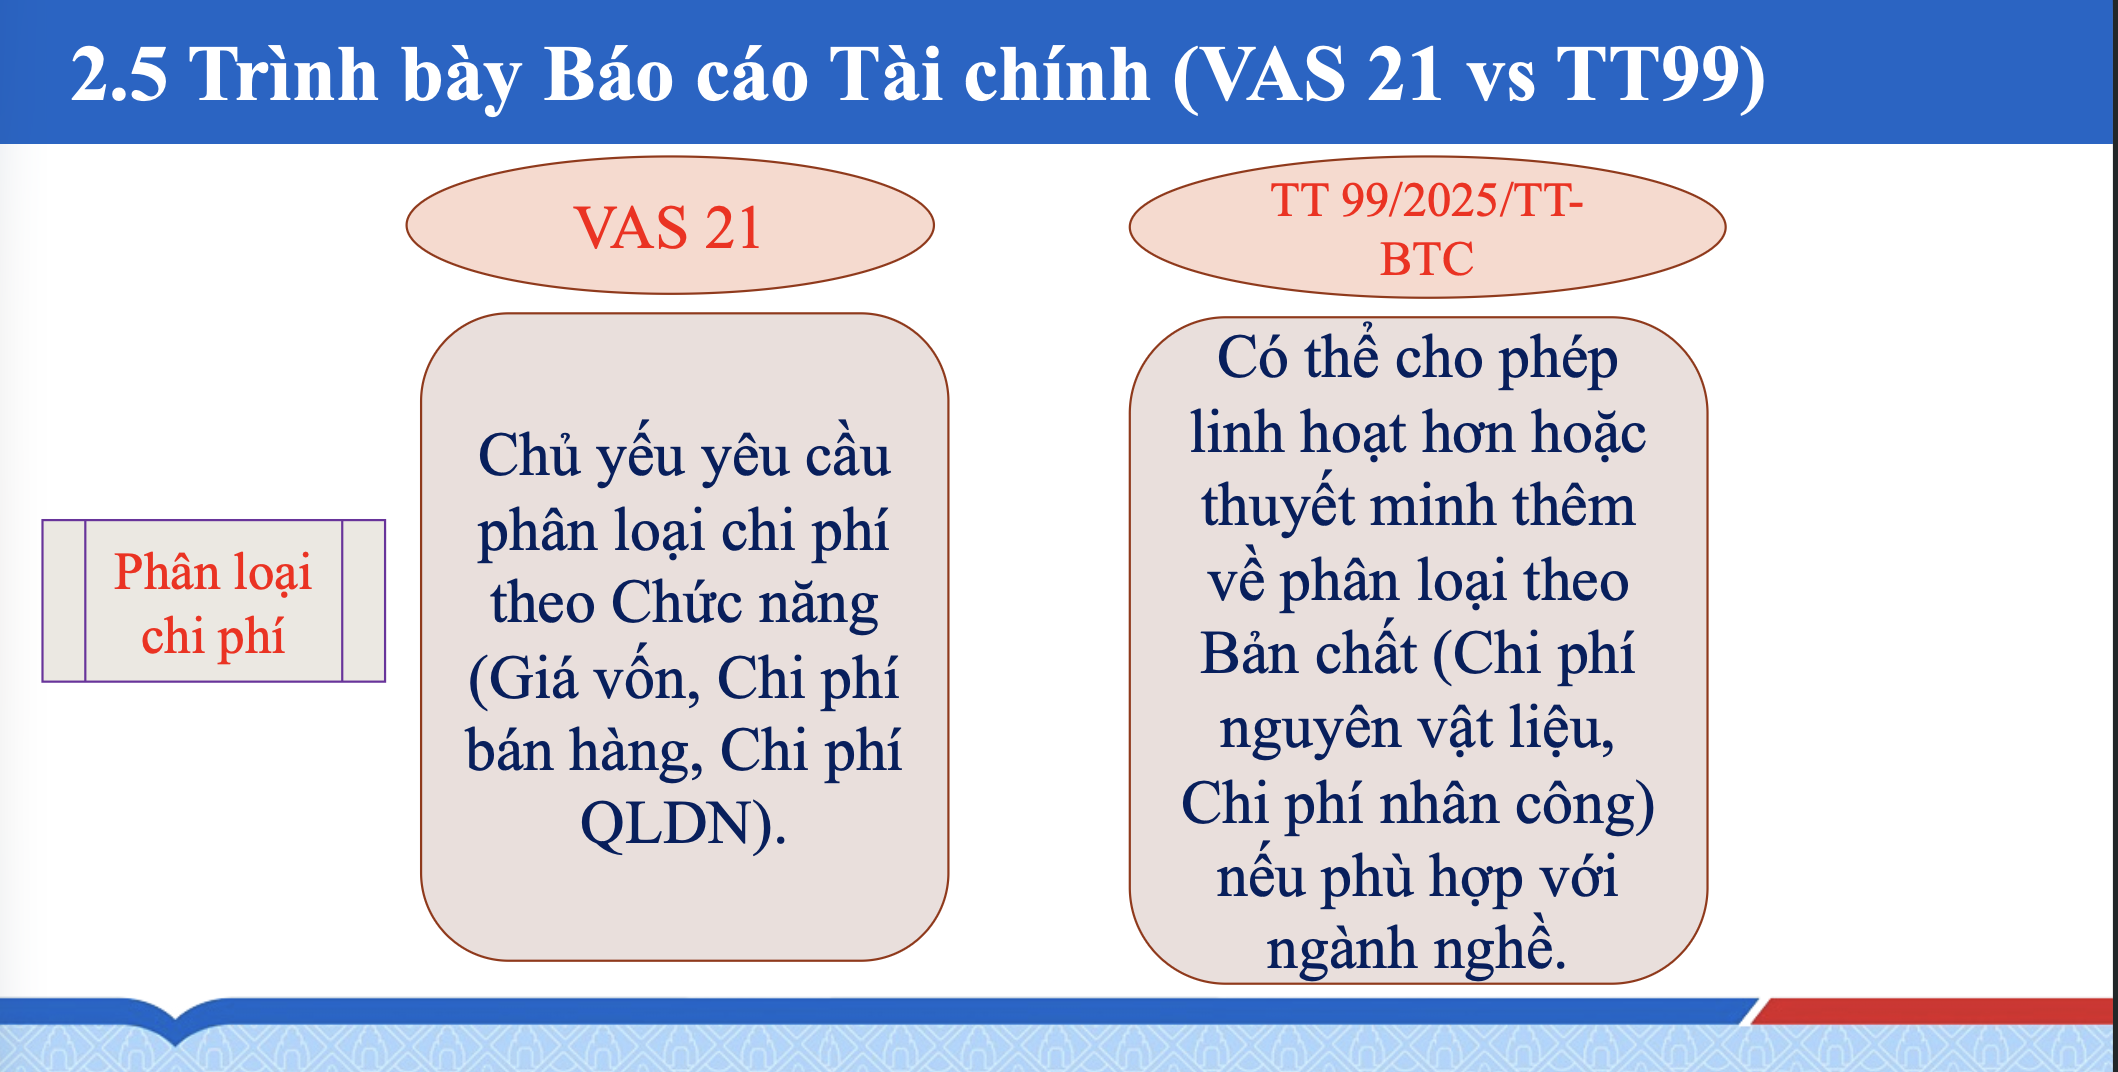
\includegraphics[width=\linewidth]{source_1.png}
    \caption{Slide --- source}
  \end{subfigure}\hfill
  \begin{subfigure}[t]{0.3\textwidth}
    \centering
    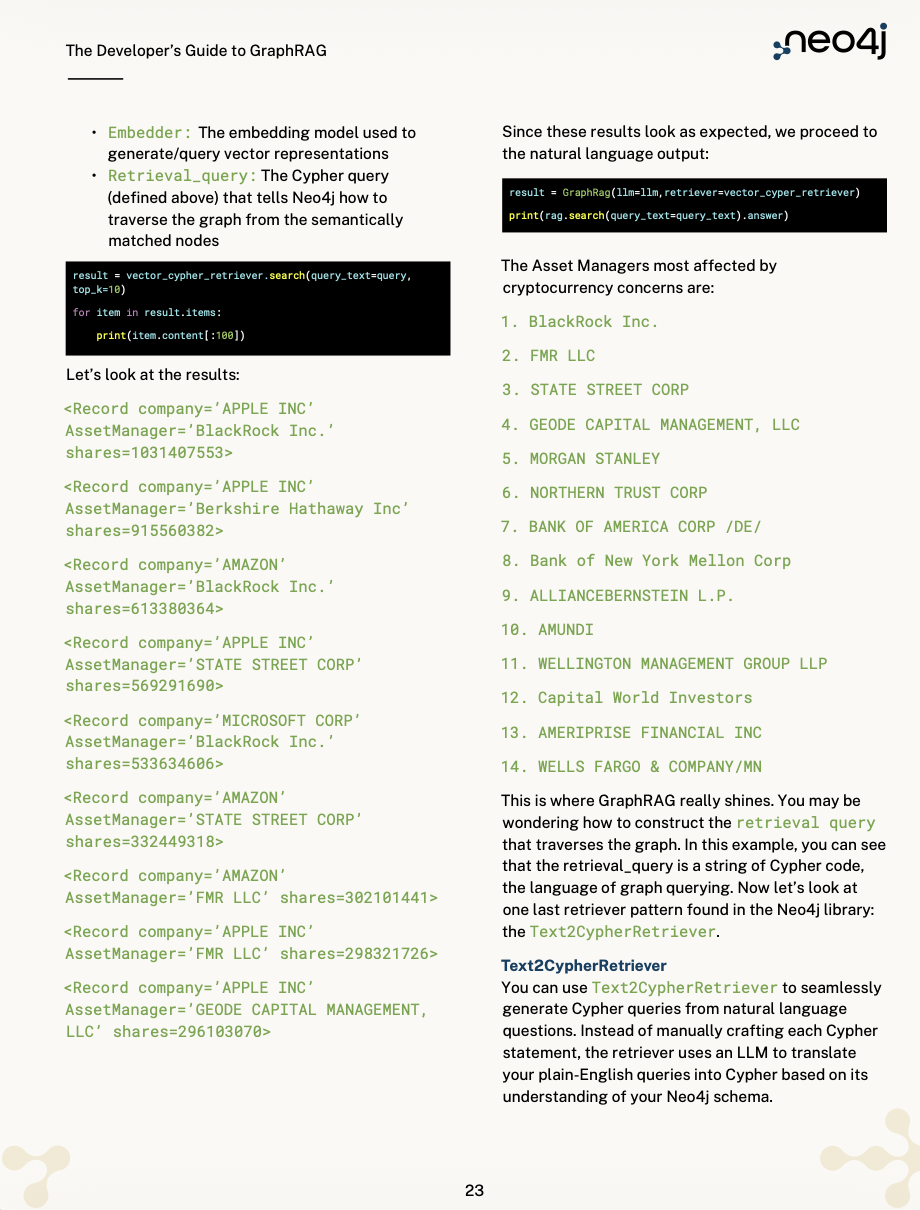
\includegraphics[width=\linewidth]{source_3.png}
    \caption{Book --- source}
  \end{subfigure}\hfill
  \begin{subfigure}[t]{0.3\textwidth}
    \centering
    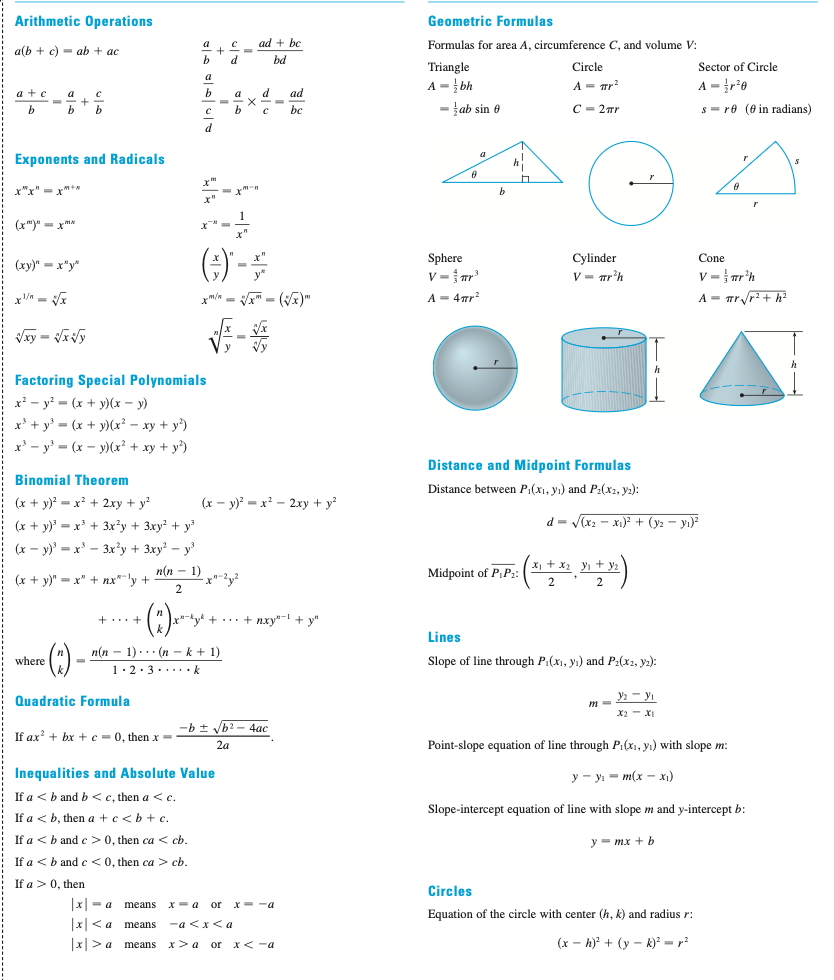
\includegraphics[width=\linewidth]{source_math.png}
    \caption{Mathematics --- source}
  \end{subfigure}

  \vspace{0.6em}

  \begin{subfigure}[t]{0.3\textwidth}
    \centering
    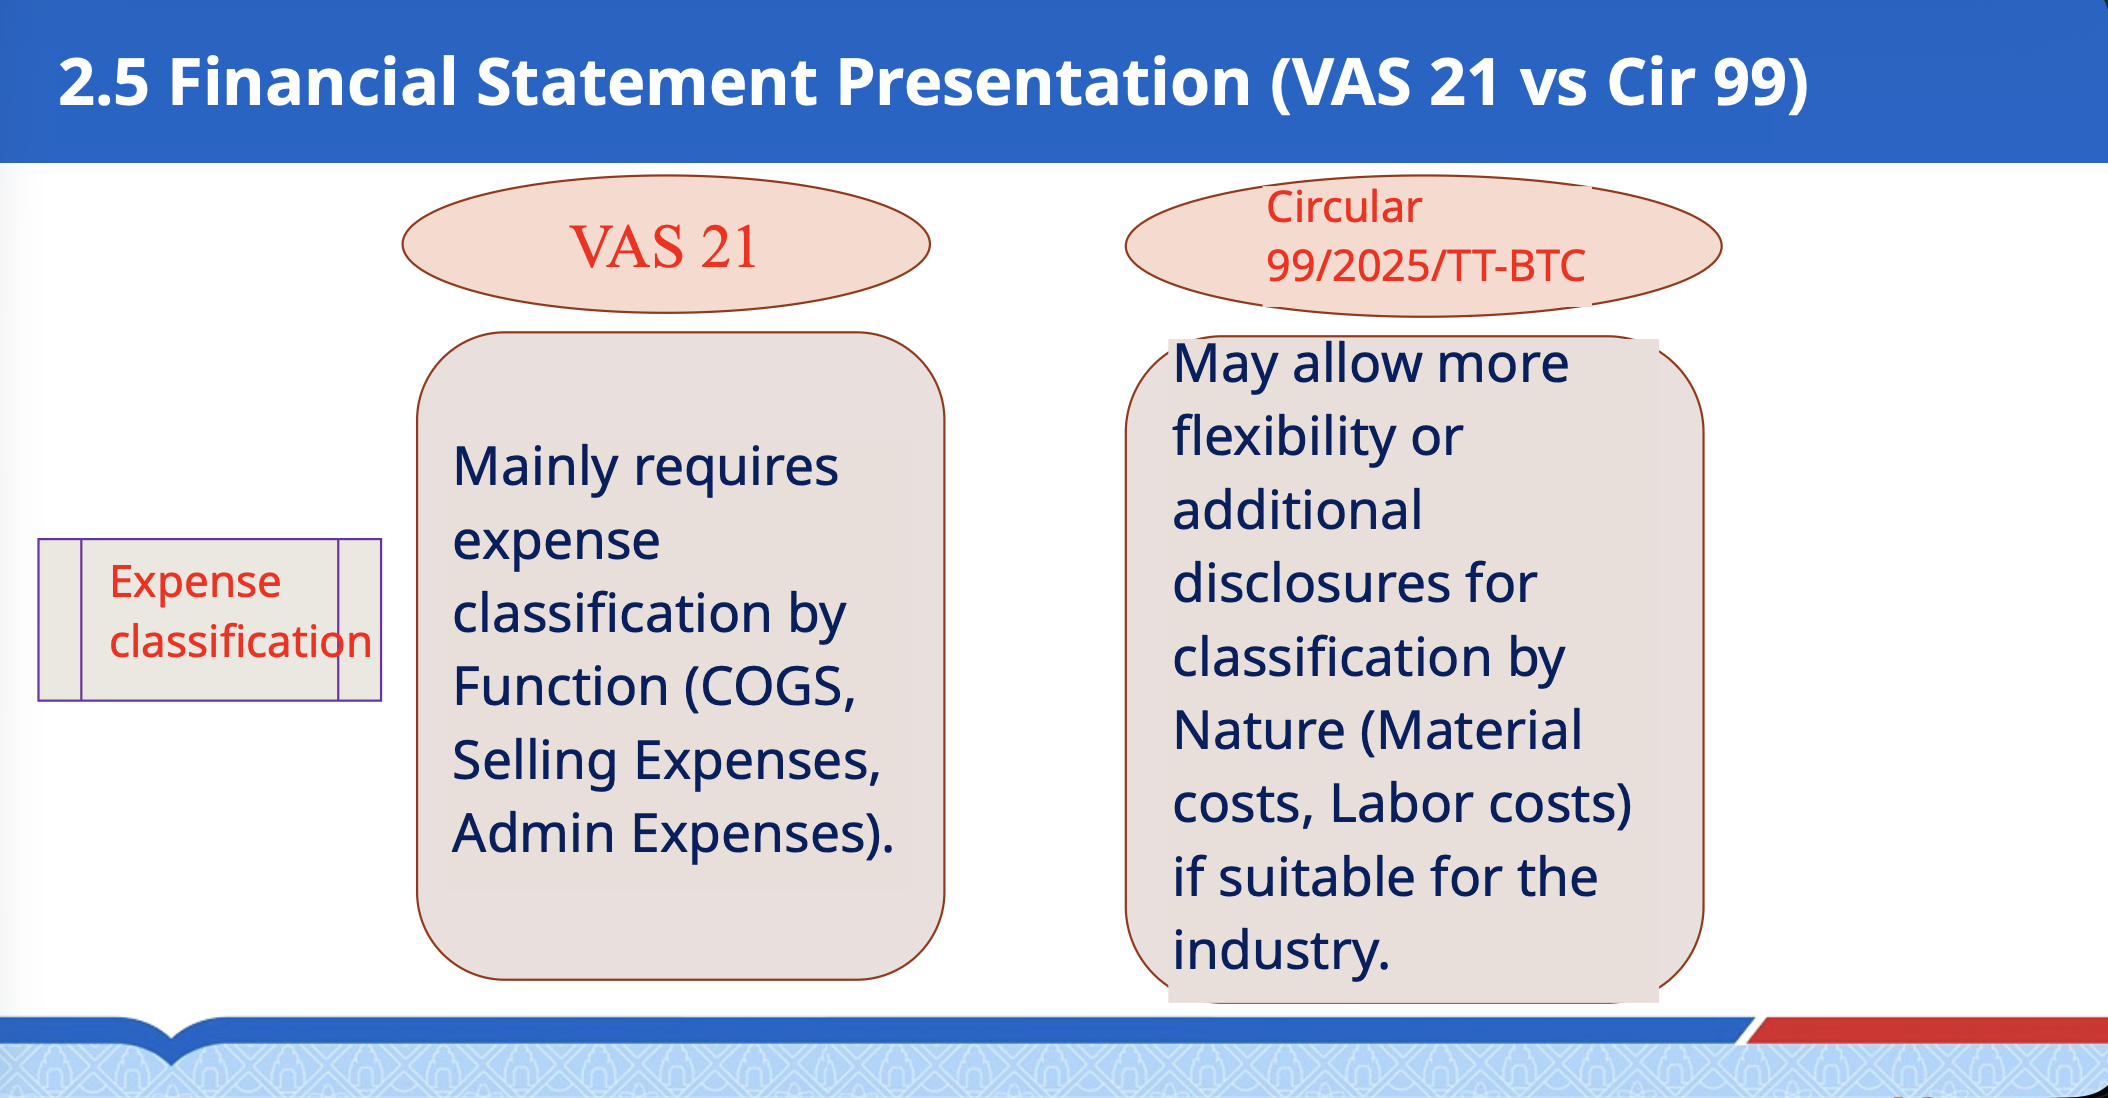
\includegraphics[width=\linewidth]{des_1.png}
    \caption{Slide --- translated}
  \end{subfigure}\hfill
  \begin{subfigure}[t]{0.3\textwidth}
    \centering
    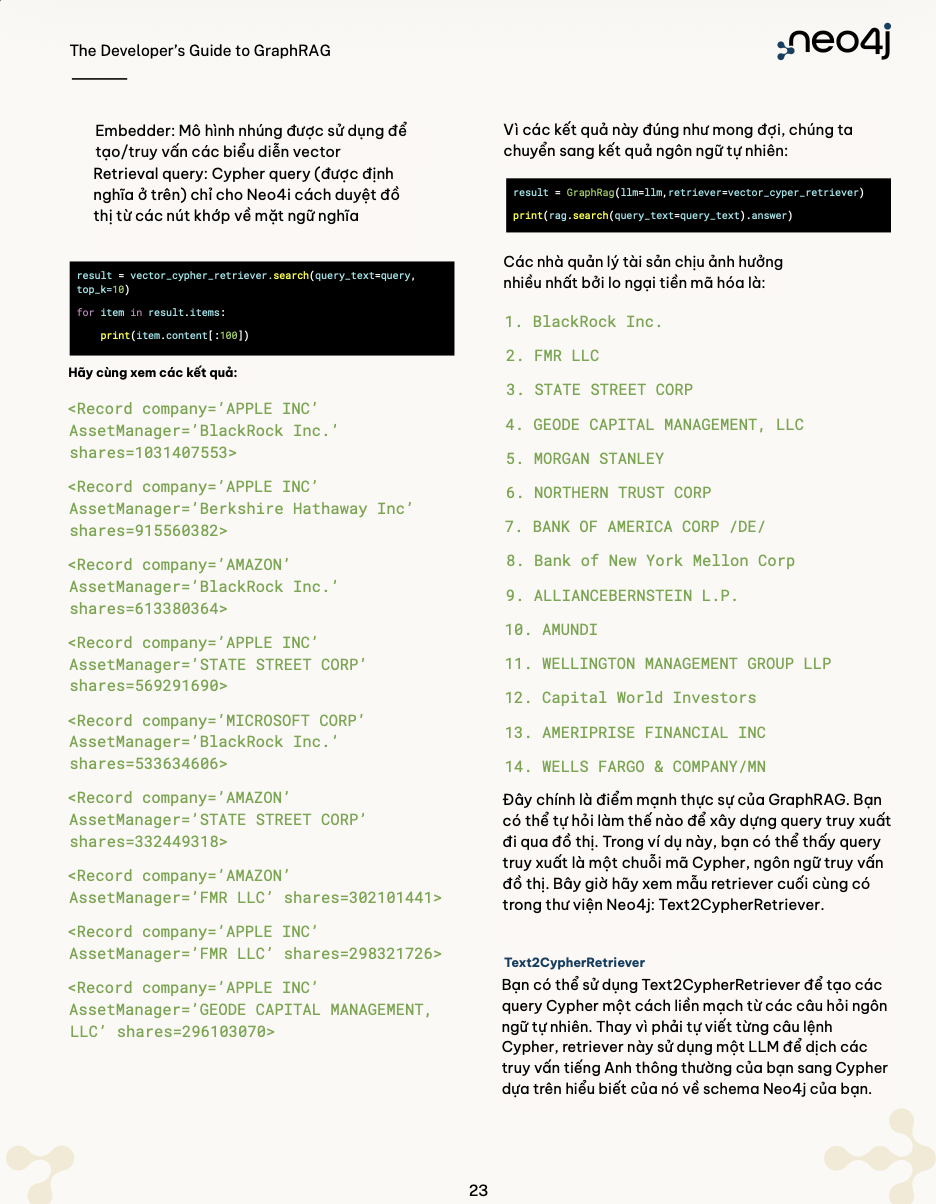
\includegraphics[width=\linewidth]{des_3.png}
    \caption{Book --- translated}
  \end{subfigure}\hfill
  \begin{subfigure}[t]{0.3\textwidth}
    \centering
    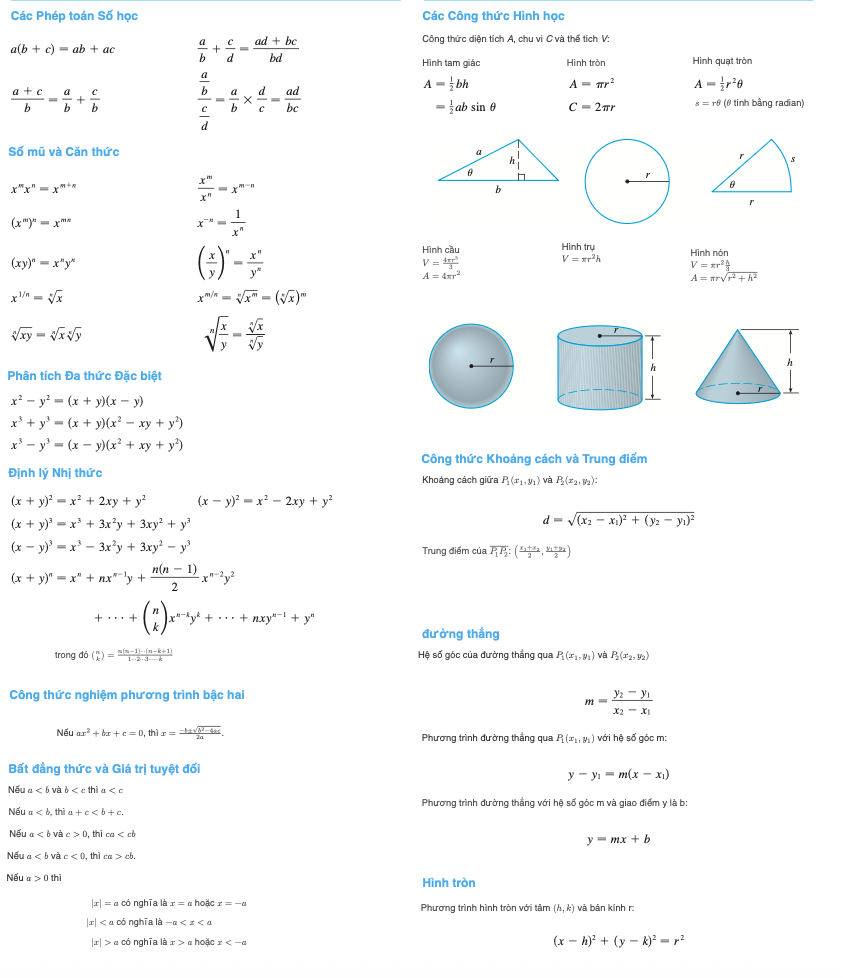
\includegraphics[width=\linewidth]{des_math.png}
    \caption{Mathematics --- translated}
  \end{subfigure}
  \caption{End-to-end output on three document genres. Top row: source pages.
  Bottom row: the corresponding pages produced by the pipeline.}
  \label{fig:qualitative}
\end{figure}

\section{DISCUSSION}
\label{sec:discussion}

The results support the two-part hypothesis, but only as stage-level evidence.
They identify where this implementation is likely constrained and what kind of
future end-to-end benchmark is needed; they do not yet prove superiority over
other PDF translation systems.

\subsection{H1: What Kind of Error Bounds the Pipeline}
\label{subsec:disc-structure}

The parsing results make a useful distinction between benign structure changes
and unrecoverable loss. Over-segmentation is visible in the gap between strict
COCO 1-1 localisation and the granularity-invariant $N$--$M$ matcher, but it is
mostly compatible with the downstream contract: fragments can be gathered,
ordered and translated as long as their text and geometry remain present. A
box-exact metric alone would therefore select against a design choice that is
helpful for translation, especially around sparse formula blocks.

The errors that matter are different. A missed region supplies no text to the
translator; a missed formula or table removes structured content; and OCR errors
turn into fluent but wrong source strings. These failures are concentrated in
specific slices---degraded historical pages, CJK OCR, three-column formulas and
table coverage---which makes them actionable. The appropriate response is not a
uniformly larger translator, but targeted parser/OCR improvements and a review
checkpoint exactly where loss first occurs.

The translation experiment gives the other half of H1. The five evaluated LLMs
do differ, but their mean COMET-DA scores occupy a narrow band compared with the
variation across target languages. That means model choice is still worth doing,
but it is a smaller controllable lever than the document-specific stages once a
competitive hosted model is used. The strongest next test of H1 is therefore
direct: improve the failing parser slices and compare the end-to-end effect
against switching translation models.

\subsection{H2: Layout Belongs to Reconstruction}
\label{subsec:disc-constraint}

The length-compliance results show why layout preservation should not be
delegated to the translator. A character budget is weakly followed and mostly
tracks target-script density: CJK output is too short by character count even
when adequacy is high, while some Latin-script targets violate by expansion.
Because the correlation with COMET-DA is effectively zero, compliance is not a
useful proxy for semantic quality.

More importantly, a character count is not the quantity the PDF cares about. The
actual layout question is whether rendered text, in the chosen font, at a local
position, collides with neighbouring elements or remains readable after
shrinking. Only the reconstruction stage has the page geometry and pixels needed
to answer that. The pipeline's size and colour decisions therefore belong in
reconstruction: size is changed only when rendered overflow would collide, and
appearance is sampled from the source page instead of assumed to be black text on
white background.

\subsection{Metric Design}
\label{subsec:disc-metrics}

The parser evaluation intentionally uses several metrics because each one
answers a different failure question. Localisation asks whether the region is
available at all; classification asks whether the right policy is applied; OCR
asks whether the translator receives the right string; reading order asks
whether context is preserved; formula CDM separates rendered mathematical
equivalence from LaTeX spelling; and table-content scoring acknowledges that
cell structure cannot be judged without cell-level ground truth. Reported
together, these metrics describe how an error would propagate through the
pipeline rather than compressing incompatible failures into one score.

\subsection{Limitations and Next Steps}
\label{subsec:disc-limitations}

Several limits remain. First, the study is not an end-to-end decomposition of
final PDF quality. It measures the parser and translator separately, then uses
the pipeline mechanism to argue which errors are recoverable. Second, final
layout fidelity is shown qualitatively but not scored with an output metric such
as overflow rate, font-shrink rate, colour error, visual similarity or
page-count preservation. Third, no direct baseline is run against systems such
as PDFMathTranslate, docutranslate or RetainPDF under one shared input and output
contract. Fourth, the cell stage is now scored, but only for geometry and only on cropped
scientific tables: no public corpus provides full pages, cell boxes that cover blank
cells, and annotations free of the over-segmentation that affects earlier datasets. Cell
geometry and table detection are therefore measured on different corpora, and logical
structure is not measured at all, because the parser does not produce it. Finally,
the experiments focus on \texttt{en}$\rightarrow$\texttt{xx}; other source
languages and document genres remain open.

The next benchmark should therefore be an annotated set of real PDFs containing
flowing text, tables, formulas, scanned pages and born-digital pages. It should
score both adequacy and final artifact quality, compare direct PDF-translation
systems and conversion-based pipelines under the same reconstruction contract,
and test whether improving parser coverage changes the final PDF more than
changing the translation model. That is the measurement needed to turn the
stage-level ordering argued here into an end-to-end claim.

\section{CONCLUSION}
\label{sec:conclusion}

This paper framed layout-preserving PDF translation as a three-stage document
problem rather than a translation problem with a rendering tail. The implemented
pipeline analyses pages visually, translates addressable elements under an
identifier contract, and reconstructs the PDF with font-size and colour
decisions computed from the source page.

The stage-level evidence supports that framing. On OmniDocBench, the parser
recovers regions well under a granularity-invariant matcher, labels them
reliably, and preserves reading order; its harmful failures are the regions,
formulas, tables and OCR slices that never reach translation correctly. On
WMT24++, competitive LLMs differ less by model choice than target languages
differ from one another. Finally, a prompt-level $\pm15\%$ character-length
constraint is weakly obeyed and uncorrelated with adequacy, so layout fidelity
must be enforced by reconstruction rather than by the translator.

The work leaves one main task: evaluate complete translated PDFs on a shared
real-document benchmark, with metrics for adequacy, overflow, readable font
size, colour fidelity, visual similarity, table-cell accuracy and runtime. That
benchmark would show whether the stage-level bottleneck identified here becomes
the dominant end-to-end bottleneck in practice.


\section*{Data availability}
The evaluation data are drawn from the public datasets cited in the manuscript.
The derived evaluation splits, annotations, and analysis code will be deposited
in a public repository. The permanent repository identifier must be inserted
before submission.

\section*{Declaration of generative AI and AI-assisted technologies in the
manuscript preparation process}
During the preparation of this work, the authors used OpenAI Codex to assist
with language editing, manuscript formatting, and consistency checks. The
authors reviewed and edited the resulting material and take full responsibility
for the content of the article.

\bibliographystyle{elsarticle-harv}
% These works are cited in the separately submitted Supplementary Material.
\nocite{fasttext,comet22,exponential-backoff,aws-backoff-jitter,
api-rate-limit-design}
\bibliography{references}

\end{document}
